\section{Introduction}
\label{sec:generalisation_intro}
Recent years have seen significant advancements in the use of deep learning for the dermatological classification of skin lesion images~\citep{du2020ai,wu2022skin}. Deep learning classifiers have been shown to be particularly effective with large datasets, such as the ISIC archive, which have enabled substantial progress in this field~\citep{tschandl2018ham10000,wen2021characteristics}. Studies utilizing high-quality datasets have reported performance that is comparable to or surpasses that of dermatologists in the classification of skin lesions~\citep{esteva2017dermatologist,haenssle2018man,han2018classification,tschandl2019expert}. Additionally, research has investigated the ability of deep learning classifiers to accurately classify macroscopic clinical images, as opposed to solely dermoscopic images~\citep{fujisawa2019deep}. However, it should be noted that images acquired from primary care settings are often of variable quality, with wider and less consistent fields of view, and may include visual distractions.

Current deep learning classifiers for medical images have been observed to exhibit poor generalization across different healthcare systems, acquisition protocols, and patient populations. This phenomenon has been documented in several studies, with evaluations typically being conducted in an internal manner, where the model training and testing datasets are drawn from the same source (e.g., \cite{han2018classification}). However, there remains a significant degree of uncertainty regarding the ability of these models to generalize across diverse domains, datasets, and imaging modalities. 

Given the complexity of the medical imaging domain, it may be unrealistic to expect the development of a universally applicable skin lesion classifier. A more practical approach may involve the utilization of local datasets to adapt models to specific target populations and healthcare systems. This approach would involve leveraging the knowledge acquired from these datasets to fine-tune existing models, thus increasing their applicability and performance within specific domains. This approach has been proposed in several studies and is considered a more realistic and practical solution to the challenges of generalization in deep learning-based medical image analysis~\citep{glocker2022risk}. 

The phenomenon of domain shift, wherein the distribution of features in the new population diverges from the distribution of features present in the training data, has been identified as a major obstacle in the deployment of artificial intelligence systems in clinical environments. This issue has been identified as a crucial challenge in implementing artificial intelligence systems in clinical settings, as highlighted in \cite{kelly2019key}. Additionally, this weakness arising from domain shift can result in unintended consequences such as gender or racial discrimination bias~\citep{glocker2022risk}. The utilization of medical datasets for the training of deep learning models is often hindered by the lack of diversity, which is often derived from a single source with a specific population distribution. Domain shift can also occur due to differences in the image capture methods, such as differences in the intensity distribution of MRI scanners at different sites~\citep{prados2017spinal} or staining of histological slides~\citep{stacke2020measuring}. These complexities pose significant challenges in delivering artificial intelligence systems in clinical settings.

The creation and curation of labelled datasets can be a costly and time-consuming task, as highlighted in recent studies such as \cite{chin2022prepare}. To address this issue, transfer learning~\citep{weiss2016survey} has emerged as a valuable approach for utilizing knowledge acquired from large datasets in other domains and applying it to a target domain with limited data. This method has been widely adopted in the field of medical image analysis, as it allows for the fine-tuning of features learned from large datasets for use in smaller datasets within the medical domain. The effectiveness of transfer learning, however, is dependent on the similarity between the source and target domains, as well as the deep learning models utilized, as noted in studies such as \cite{matsoukas2022makes}. For instance, the utilization of knowledge acquired from the large ImageNet dataset~\citep{deng2009imagenet} has been extensively applied in medical image analysis, despite the visual dissimilarity between the images in ImageNet and medical images. This approach has been demonstrated to be effective in the deep classification of the ISIC 2019 dermoscopy dataset, with evidence of feature re-use~\citep{matsoukas2022makes}.

In this study, the effectiveness of transfer learning between dermatology datasets is investigated with a focus on the utilization of deep learning models to assist in the diagnosis of skin lesions based on community images acquired with limited control. The effectiveness of transfer learning is expected to be dependent on the size of the source datasets used for pre-training, as well as the similarity between these source datasets and the target datasets.

To explore this topic, two types of deep learning models with different inductive biases are focused on. The performance of these models is evaluated in relation to two novel datasets, specifically designed to simulate a real-world clinical setting. These datasets were gathered, trained, and tested in the context of image referrals sent to secondary-care hospital-based dermatologists from primary care. This use case was selected as it represents a common scenario in dermatology in the UK and aims to reliably identify common benign conditions in this setting.

The results from the experiments with generalisation between the different dataset generalisation shows that’s performance is based on the proximity of the training distribution to the testing distribution. Therefore, it is critical to obtain data from the specific real-world setting in which the deep learning will be deployed. By training, and testing on two datasets, one from primary care and the other from referred images sent for medical photography, aims to demonstrate that the approach is effective in a real-world clinical setting and can be used for triage experiments.

The work discussed in this chapter is yet to be published but is intended for submission to the British Journal of Dermatology, under the authorship of Jacob Carse, Gillian Chin, Charlotte Proby, Emanuele Trucco, Colin Fleming, and Stephen McKenna. The personal contribution to this collaborative effort is reflected in the experiments carried out on the generalization of the dataset.



\section{Datasets}
\label{sec:generalisation_datasets}
In this study, two datasets of community-acquired macroscopic (non-dermoscopic) images were curated. These datasets were extracted from previously stored images referred from primary to secondary care in Tayside and Forth Valley, United Kingdom. The inclusion of these datasets allows for the examination of a diverse range of macroscopic images acquired in a community setting. Both sets of images were annotated using the same procedure, explained in Section~\ref{subsec:annotation_procedure}.

\begin{figure}
	\centering
	\captionsetup[subfigure]{singlelinecheck=false}
	\begin{tabular}{ccc}
		\subcaptionbox{\centering Tayside Melanoma}{\includegraphics[width=0.3\textwidth]{images/TAY_MEL.jpg}} &
		\subcaptionbox{\centering Tayside Melanocytic Nevus}{\includegraphics[width=0.3\textwidth]{images/TAY_NV.jpg}} &
		\subcaptionbox{\centering Tayside Benign Actinic Keratosis}{\includegraphics[width=0.3\textwidth]{images/TAY_BKL.jpg}} \\
		\subcaptionbox{\centering Forth Valley Melanoma}{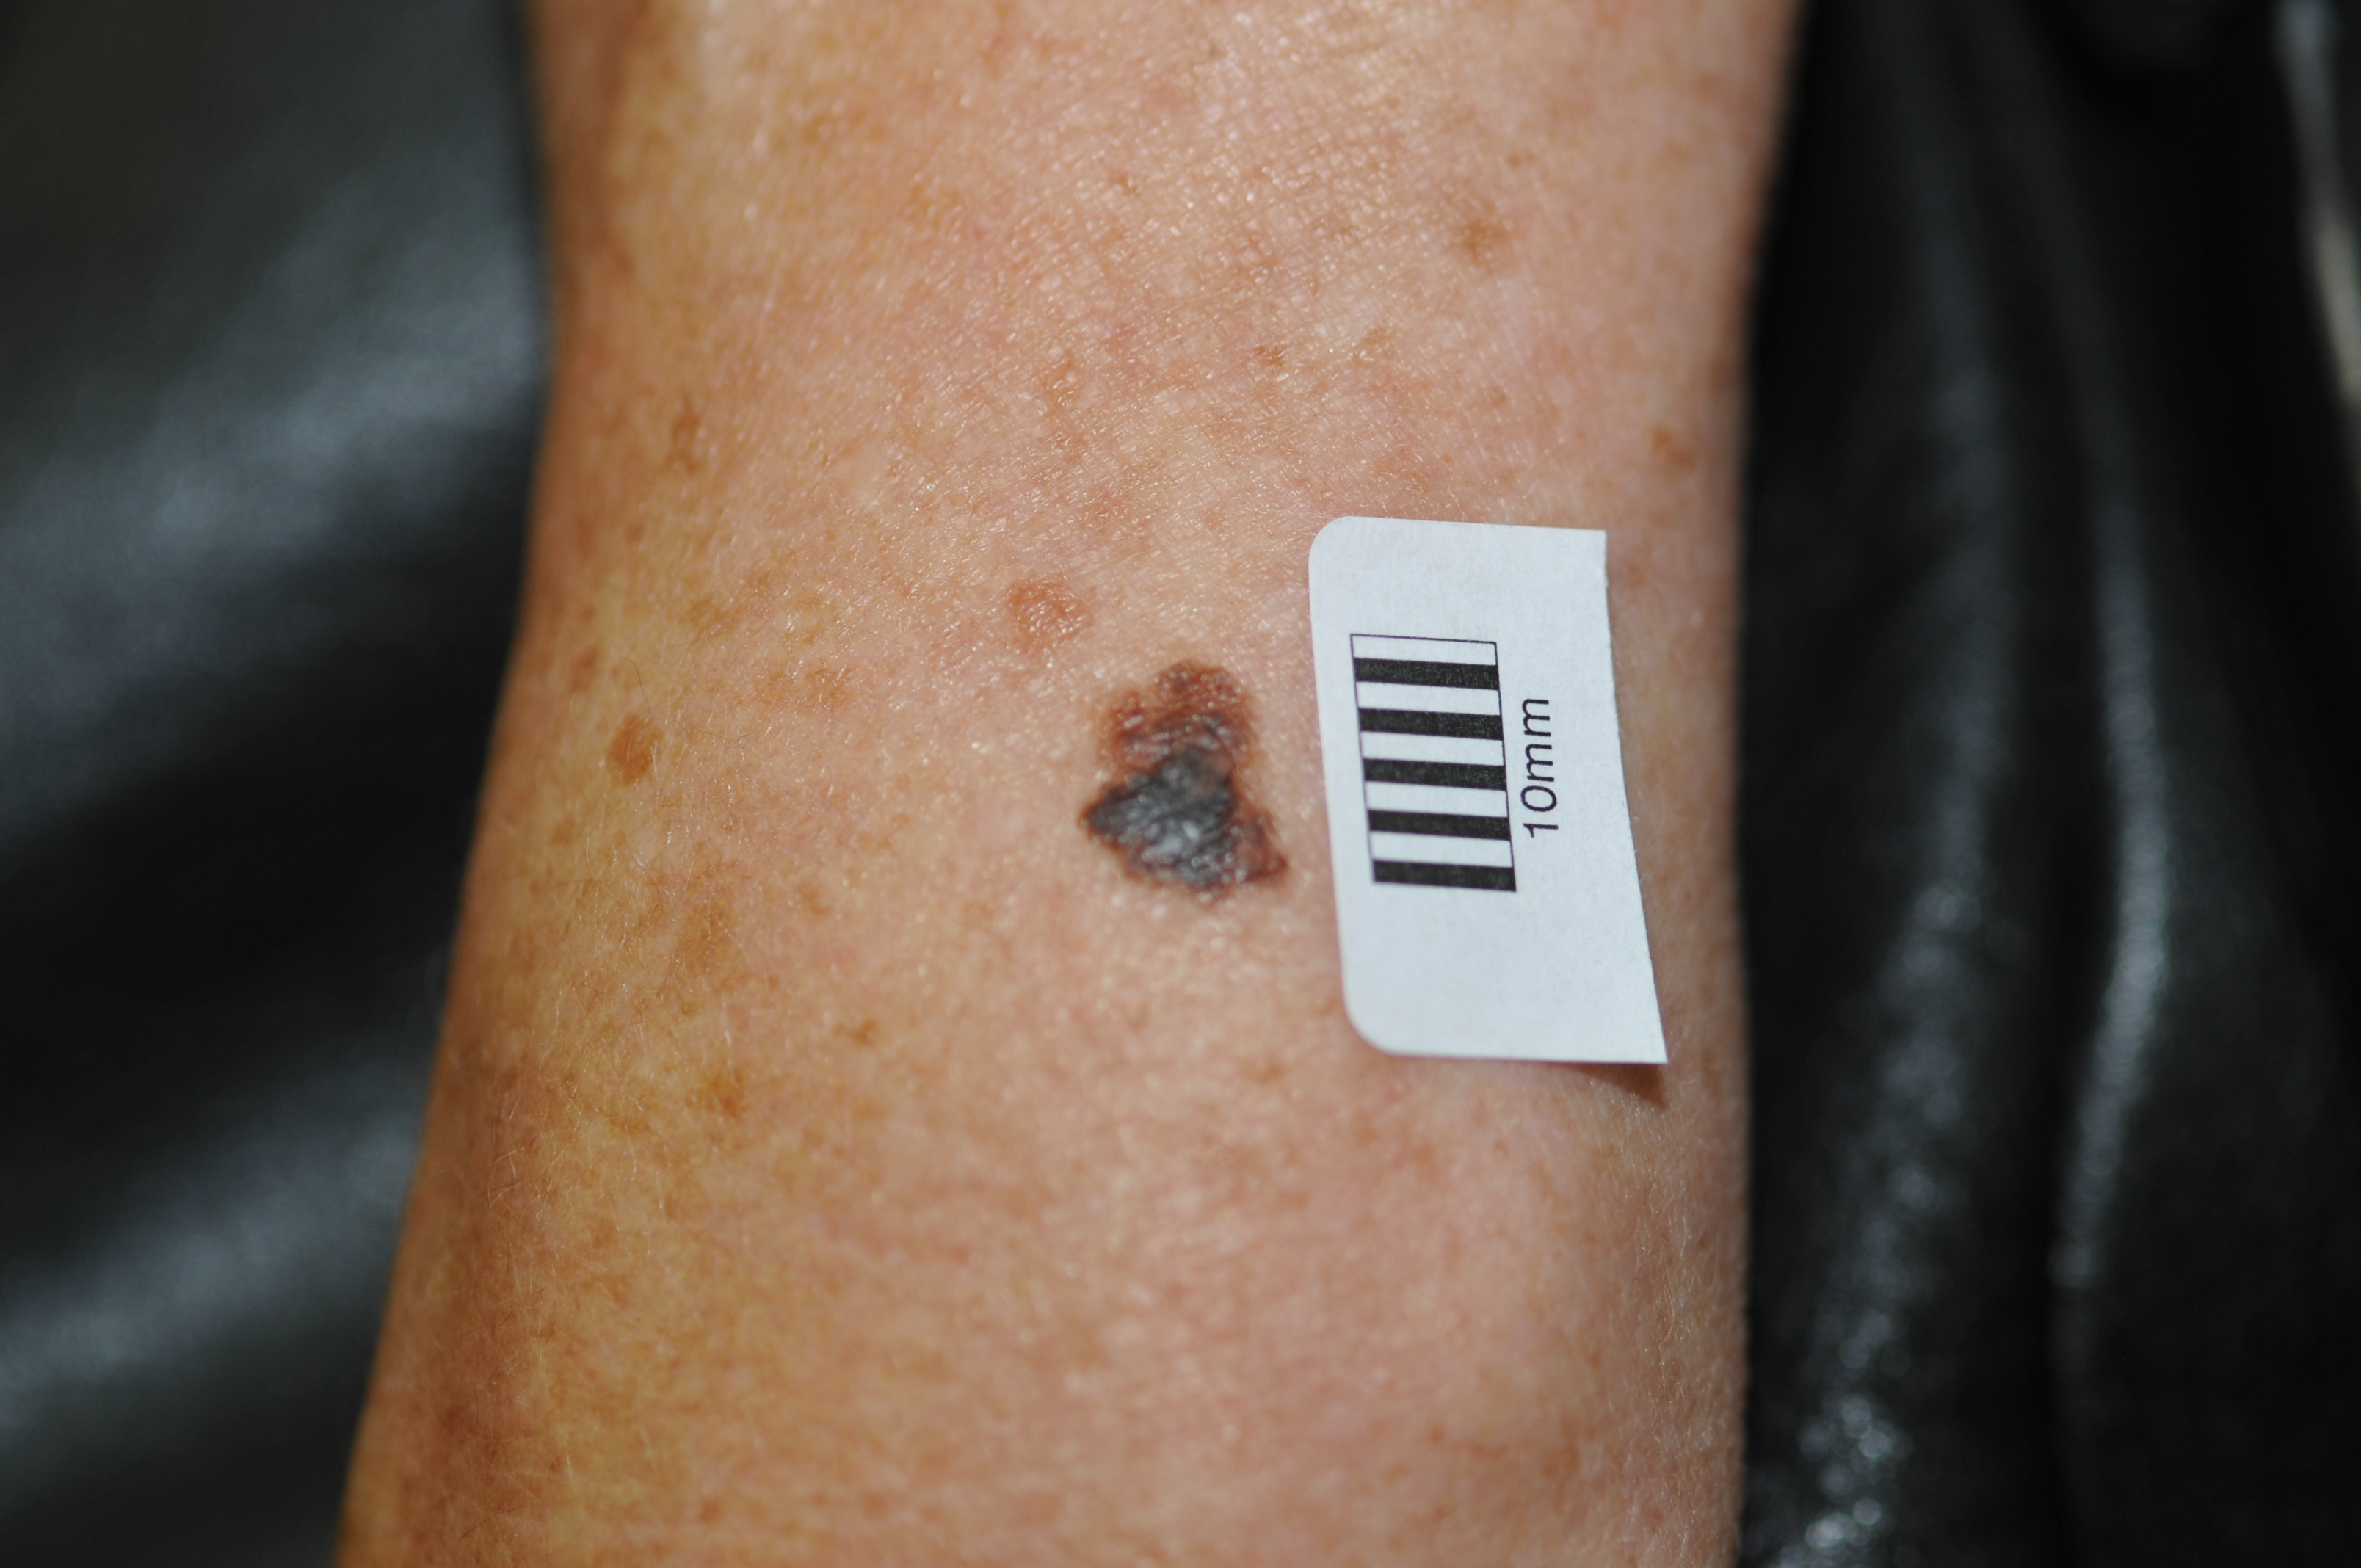
\includegraphics[width=0.3\textwidth]{images/FV_MEL.jpg}} &
		\subcaptionbox{\centering Forth Valley Melanocytic Nevus}{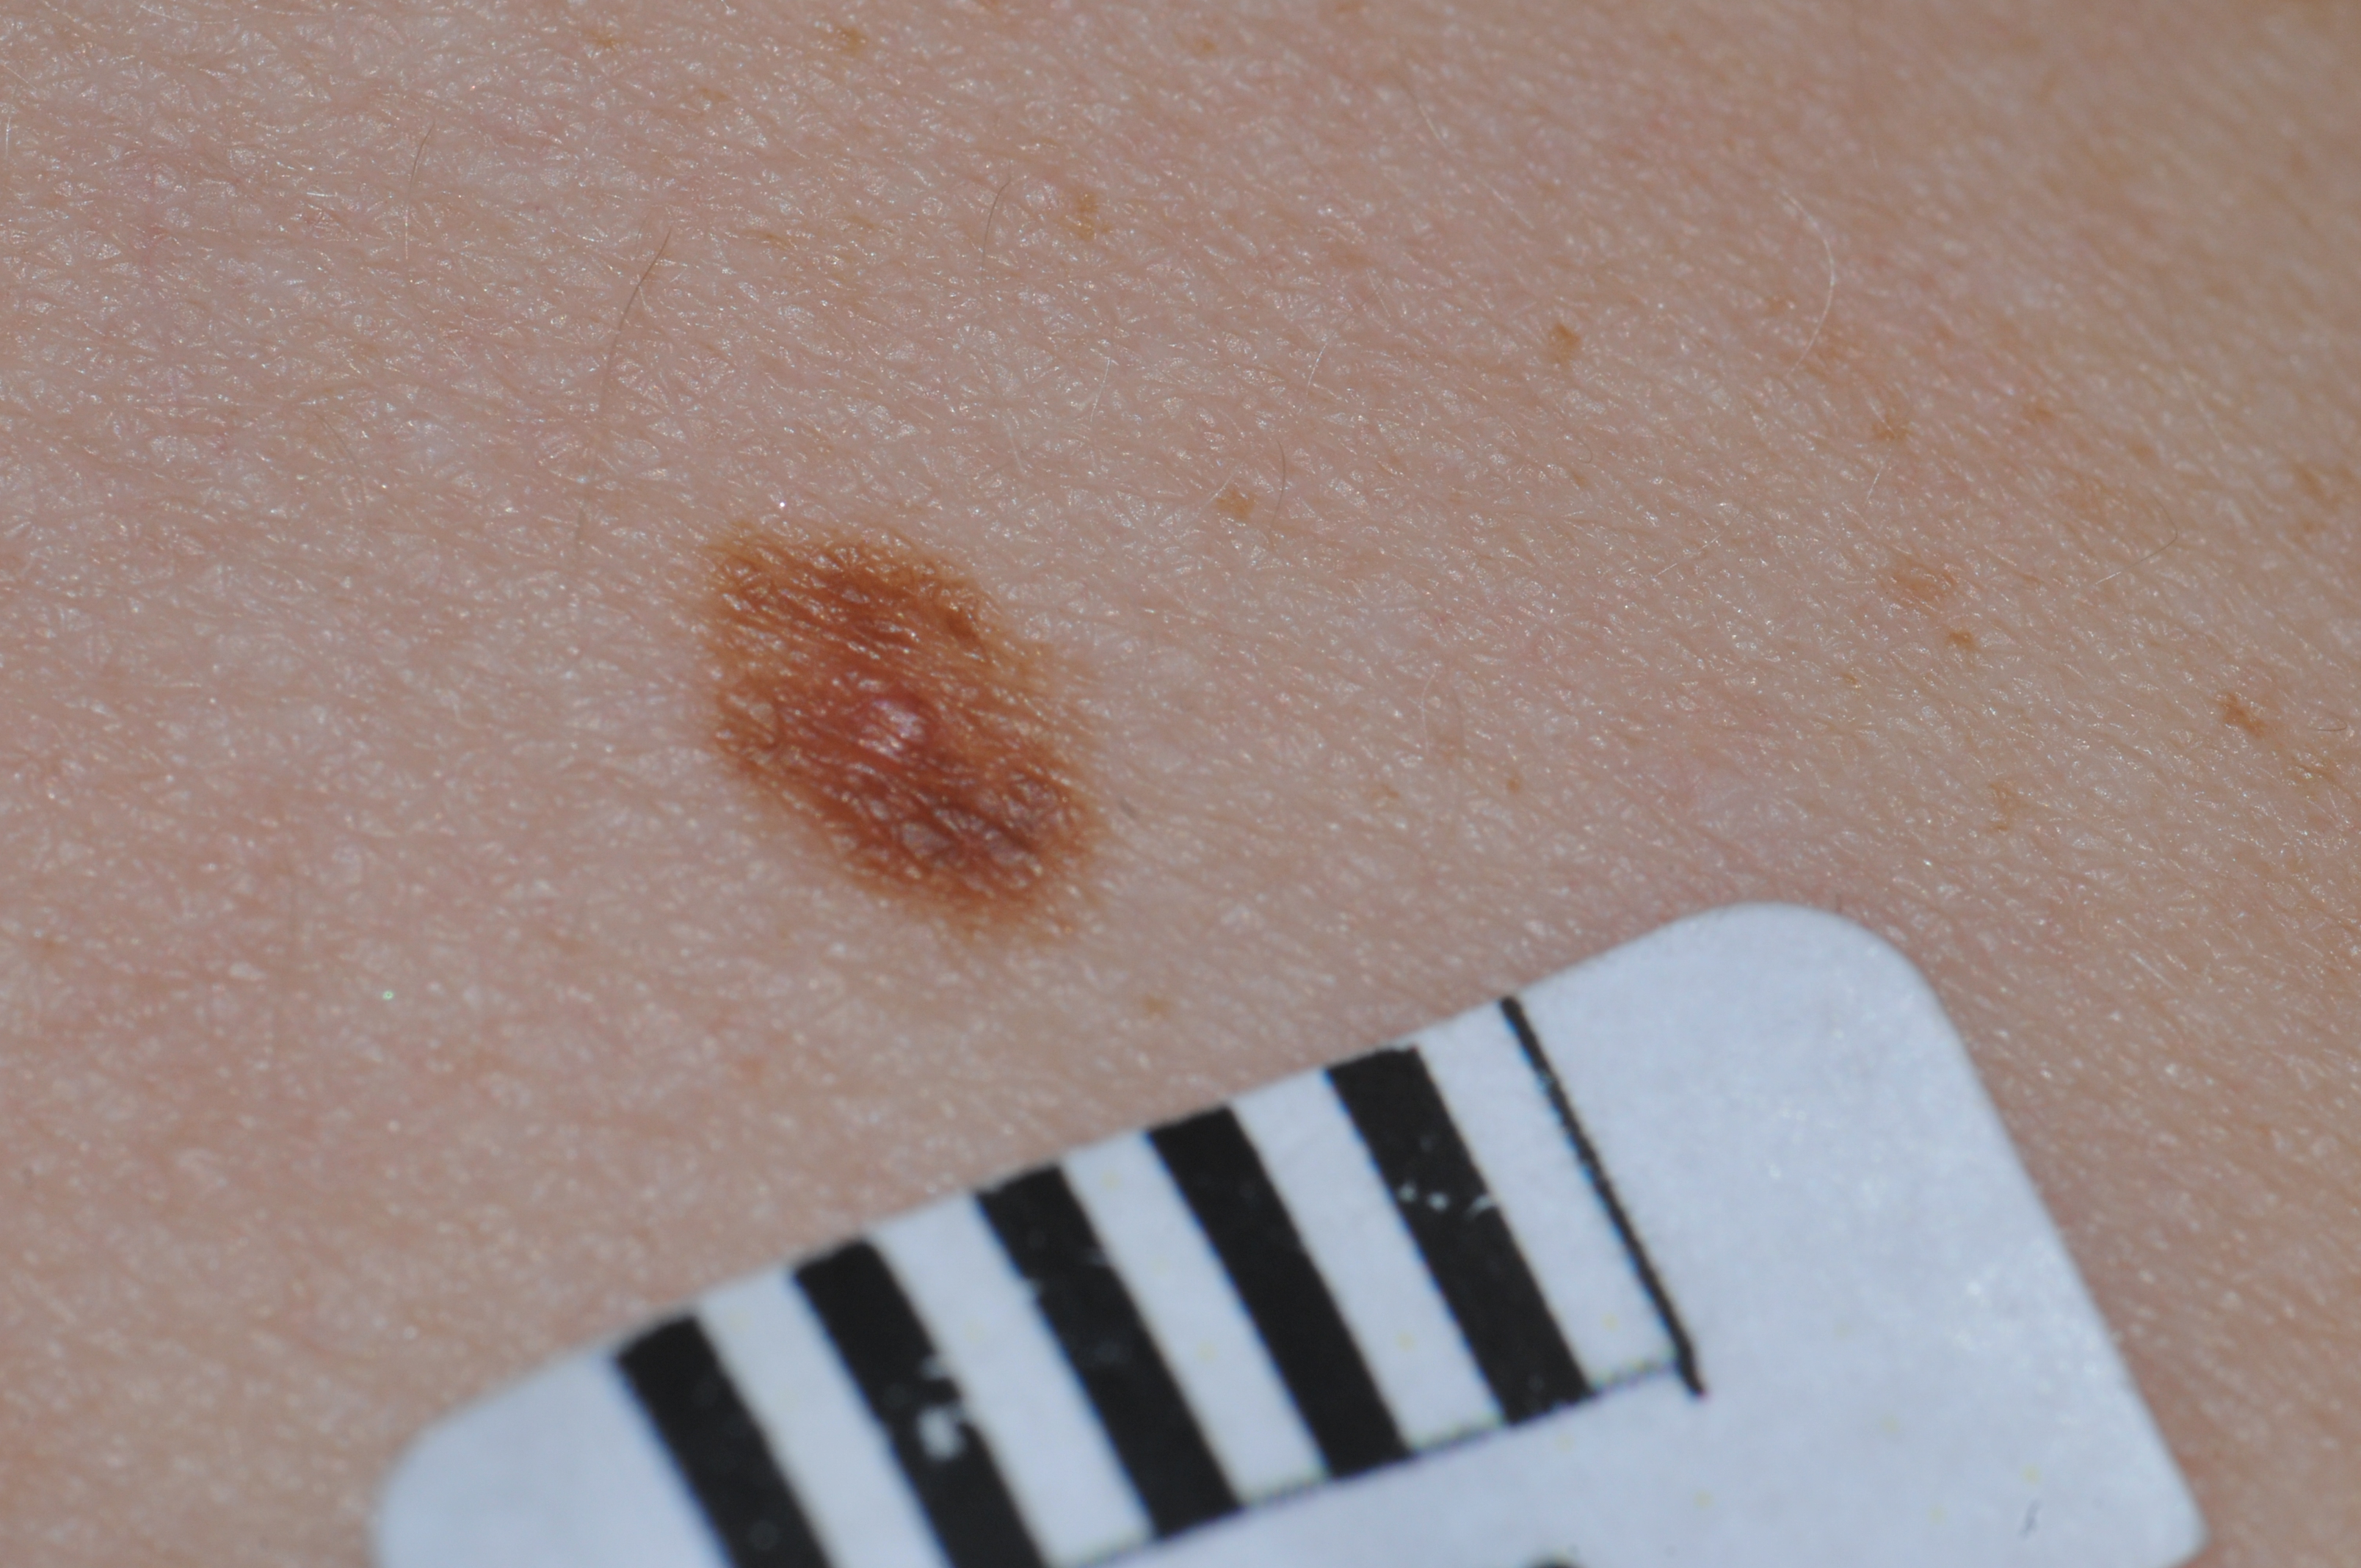
\includegraphics[width=0.3\textwidth]{images/FV_NV.jpg}} &
		\subcaptionbox{\centering Forth Valley Actinic Keratosis}{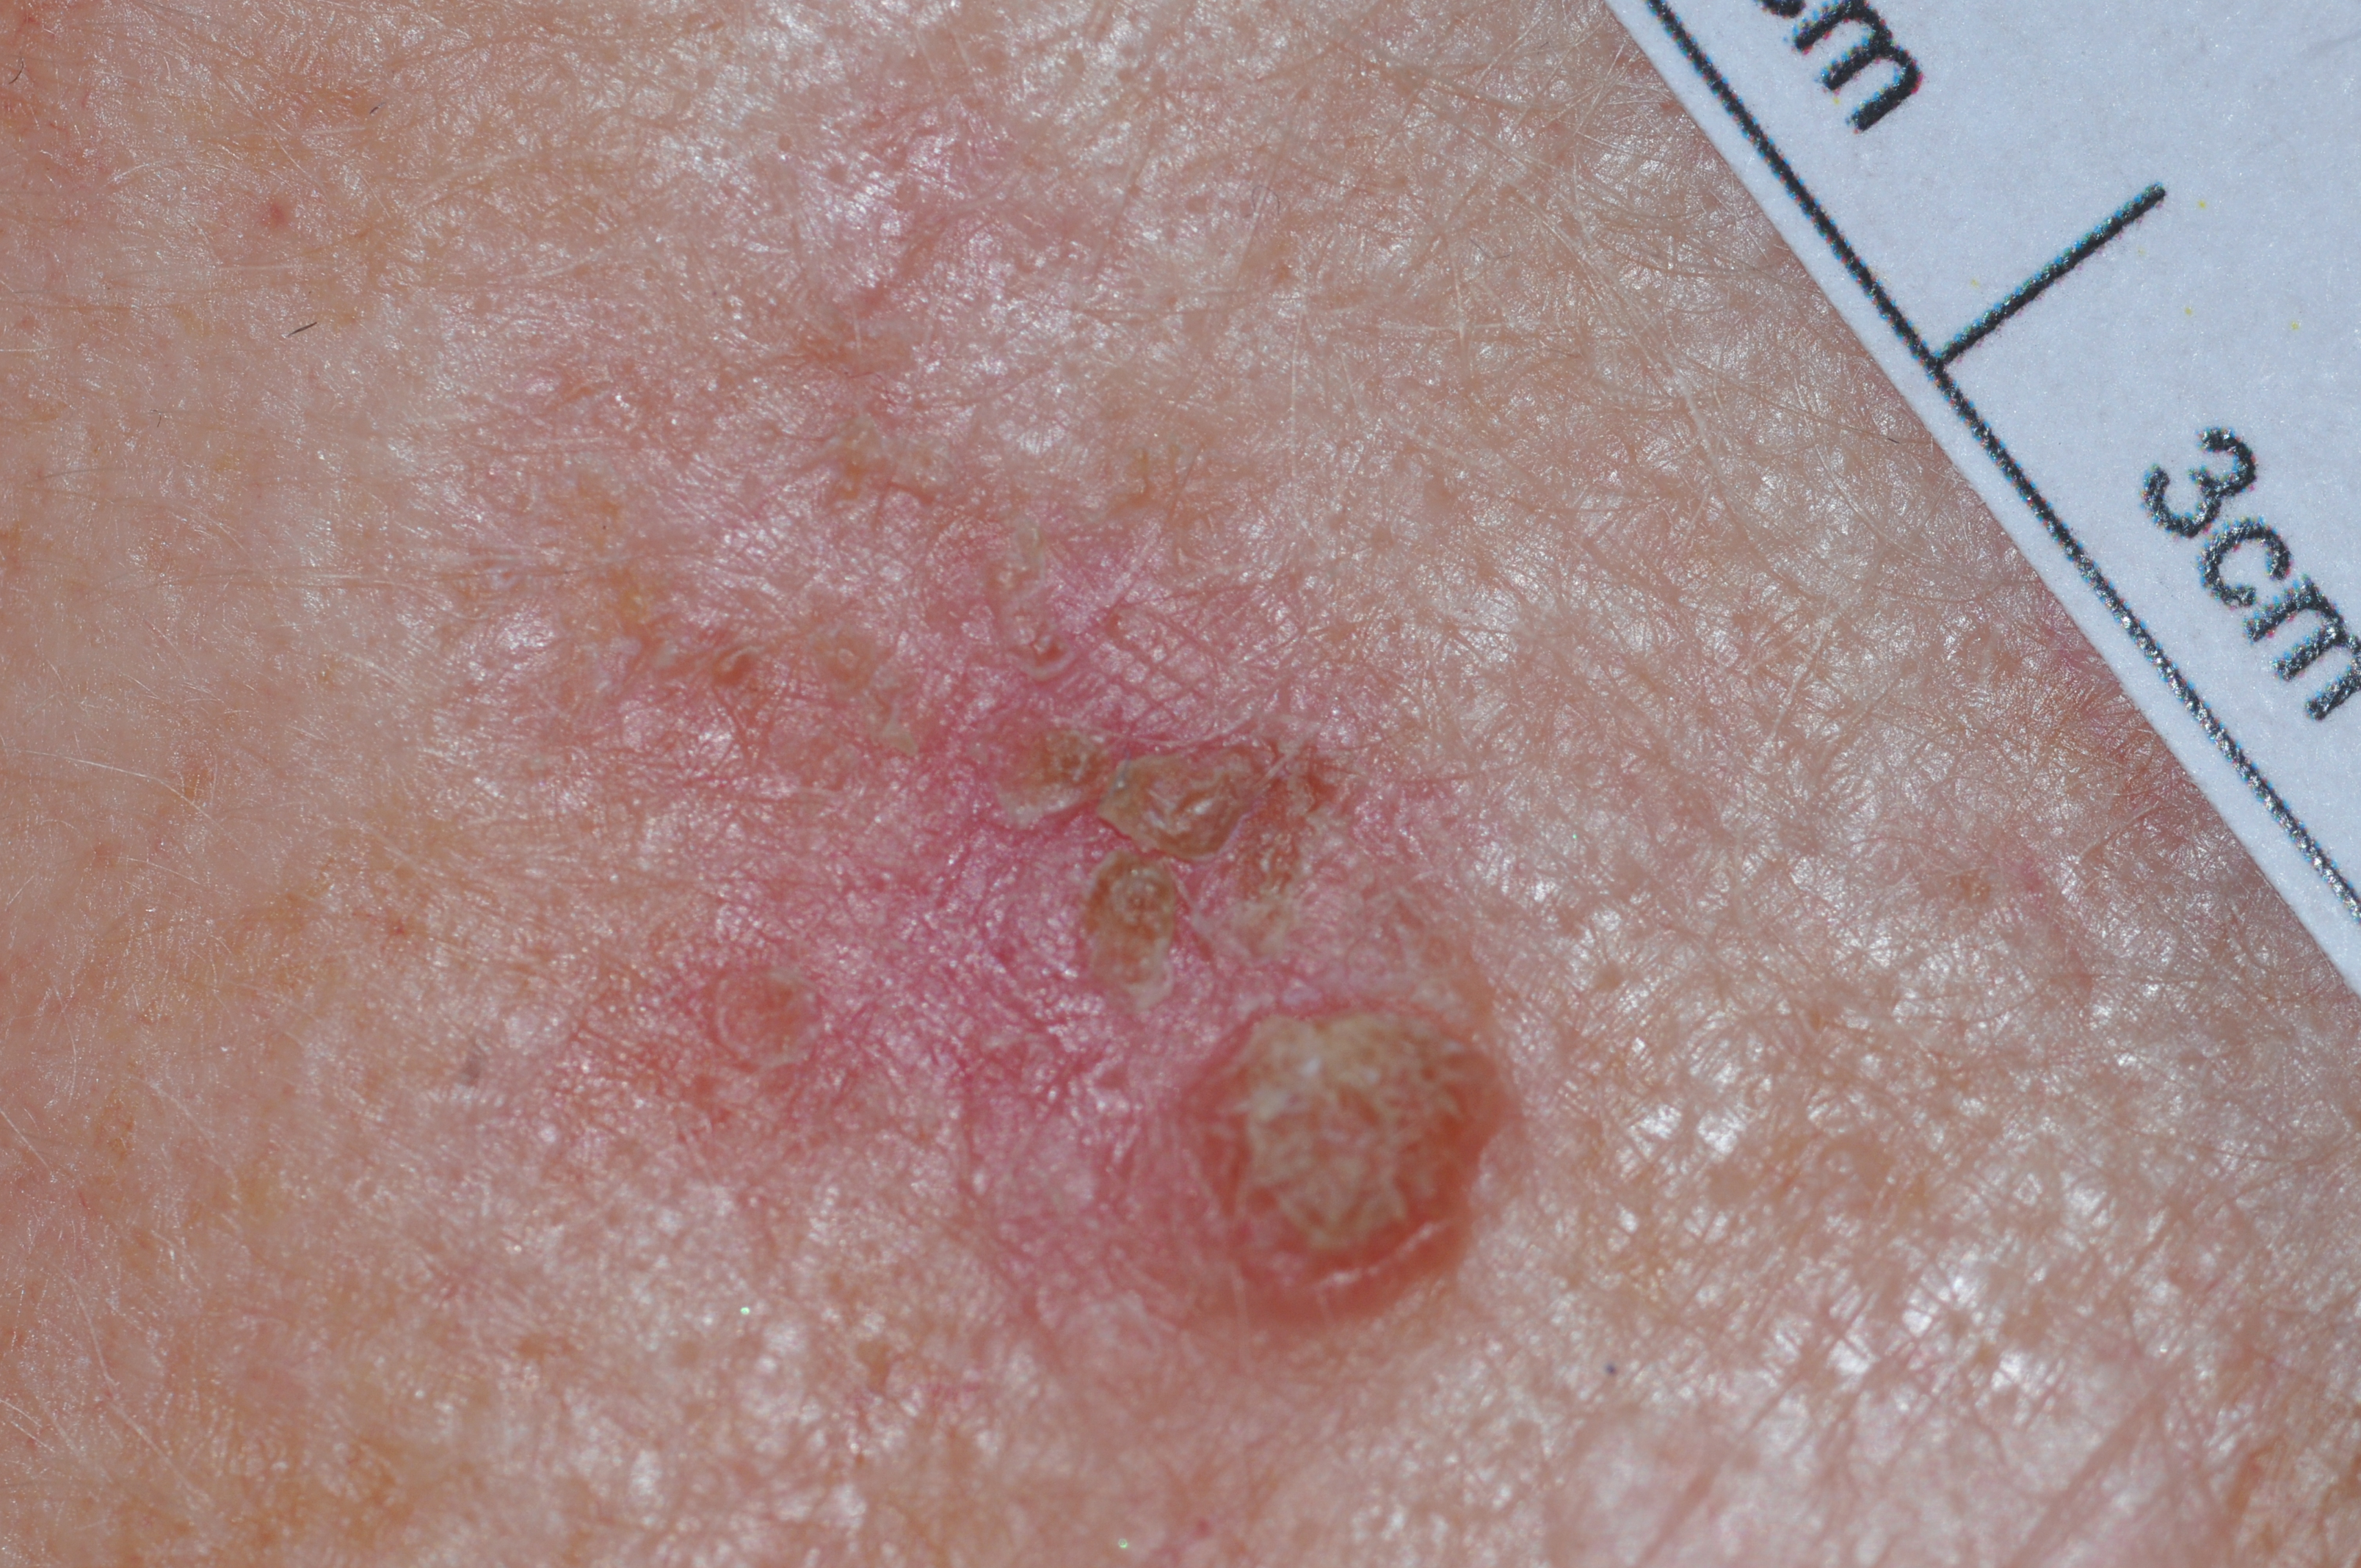
\includegraphics[width=0.3\textwidth]{images/FV_AK.jpg}}
	\end{tabular}
	\caption{Example images from the Tayside and Forth Valley datasets.}
	\label{fig:nhs_dataset_examples}
\end{figure}

\subsection{Tayside Dataset}
\label{subsec:tayside_dataset}
The Tayside dataset (collected by Professor Colin Fleming), sourced from NHS Tayside~\footnote{NHS Tayside: \url{nhstayside.scot.nhs.uk}}, is centred on community-acquired skin lesion data, that represent real-world data capture from primary care. The images were obtained by primary care practitioners utilizing a diverse array of cameras, from various cutaneous anatomical sites, utilizing non-standardized lighting, framing, focusing, and acquisition settings. The dataset is intended for triage experiments, with the goal of reliably identifying common benign conditions in a real-world clinical setting. This dataset not only represents real-world teledermatology images acquired by primary care practitioners, but it also serves as a proxy for international skin datasets, where high-quality images and dermoscopy may not be readily available.

\subsection{Forth Valley Dataset}
\label{subsec:forth_valley_dataset}
The Forth Valley dataset (collected by Dr. Colin Morton) was procured by medical photographers capturing image of patients skin lesions, who were referred by primary care practitioners for specialist assessment within NHS Forth Valley~\footnote{NHS Forth Valley: \url{nhsforthvalley.com}}. The medical photographers possess a higher degree of expertise in the acquisition of photos of skin lesions, despite potentially lacking specialized knowledge in the field of dermatology. The medical photographers employ standard equipment, such as cameras, lighting, and backgrounds, to ensure uniformity in image quality. Furthermore, a standardized pattern of image capture is utilized to ensure high-quality, wide-angle, and close-up macro images.

\subsection{Annotation Procedure}
\label{subsec:annotation_procedure}
The datasets underwent a comprehensive annotation process that adhered to strict ethical guidelines and protocols for ensuring the quality and clinical usefulness of the images. This annotation procedure developed by the Dermatology department at NHS Tayside. This included the removal of duplicate images and those that were not clinically relevant, as well as the de-identification and cropping of images to highlight any abnormalities. The images were then assigned a diagnostic label using the British Association of Dermatologists diagnostic index~\footnote{BAD Clinical Guidelines: \url{https://www.bad.org.uk/guidelines-and-standards/clinical-guidelines/}}, which corresponds to the International Classification of Diseases (version 11)~\footnote{ICD-11: \url{https://icd.who.int/dev11/l-derma/en}}. The assignment of these labels was conducted by two consultant-level dermatologists, registered on the UK General Medical Council specialist register of dermatologists~\footnote{UK GMC Medical Register: \url{https://www.gmc-uk.org/registration-and-licensing/the-medical-register/}}, and any discrepancies were resolved by a third consultant-level dermatologist. This decision was based on all available clinical information, including pathology reports from a consultant pathologist. The labels represent real sources of data, with diagnoses for malignancy being derived from pathology, and for benign lesions, based on the opinions of consultant dermatologists. The risk of serious misdiagnosis, such as mistaking malignant disease for benign disease, is less than 1 in 10,000, as per the audit experience of this group. The full annotation procedure is presented in detail for further reference.

\begin{enumerate}
	\item Ensure the necessary Caldicott/Ethical approvals are in place. 
	\item Proceed to open the first patient record.
	\item Proceed to view the images. For each image, determine whether to retain it as potentially diagnostically useful, retain as a negative control, or discard it.
	\begin{enumerate}
		\item Retain as potentially diagnostically useful if any triage-level information can be obtained from the image.
		\item Retain as negative control if a clinical image of skin without even triage level information i.e., where photographic information is insufficient to make a skin diagnosis. This may include images which are blurred by background details e.g., scarring or tattooing.
		\item Discard the image if: a. No skin clinical images present, e.g., a clinical letter with no images may be in your system, X-ray image b. Duplicate image, i.e., multiple images, of which you will choose the best single view.
	\end{enumerate}
	\item If retaining the image, anonymize where necessary. This may involve the removal of distinguishing features e.g., a tattoo, a label with patient details, or full-face views. Minimize cropping to ensure the remaining image has a maximum resolution. 
	\item Where multiple skin lesions, attempt to crop the image to ensure one lesion per image. Minimize cropping to ensure the remaining image has a maximum resolution.
	\item For multiple skin lesions of the same disease process/widespread disease, if not possible to crop sufficiently, ensure all skin lesions have the same diagnostic label and are the same disease process.
	\item Label the image with the diagnosis using BAD Diagnostic Index.
\end{enumerate}



\section{Generalisation Experiments}
\label{sec:generalisation_experiments}
This section details the datasets, training parameters, experimental setup, and results for the experiments with dermatology cross dataset generalisation. The code and full results used within this section can be found on the project GitHub repository~\footnote{GitHub Repository: \url{github.com/UoD-CVIP/Lesion-Classifier}}.

\subsection{Datasets}
\label{subsec:generalisation_datasets}
In our experiments, we utilized images from two public domain skin lesion datasets in addition to the datasets from Tayside and Forth Valley. These datasets were the ISIC 2019 dataset~\citep{codella2018skin,combalia2019bcn20000,tschandl2018ham10000} and the SD-260 dataset~\citep{yang2019self}. The ISIC datasets are among the largest publicly available, with ISIC 2019 containing over 26,000 skin lesion images labelled with diagnoses. These images were acquired using dermatoscopes, which tend to produce well-centered, zoomed in, and consistent resolution images. In contrast, the SD-260 images were acquired in less controlled environments with varying imaging devices, resulting in more variation in colour, exposure, illumination, resolution, and scale (Figure~\ref{fig:sd260_examples}). Visually, they are qualitatively similar to the Tayside and Forth Valley datasets but are acquired from a Chinese population.

\begin{figure}
	\centering
	\captionsetup[subfigure]{singlelinecheck=false}
	\begin{tabular}{cc}
		\subcaptionbox{\centering Melanoma}{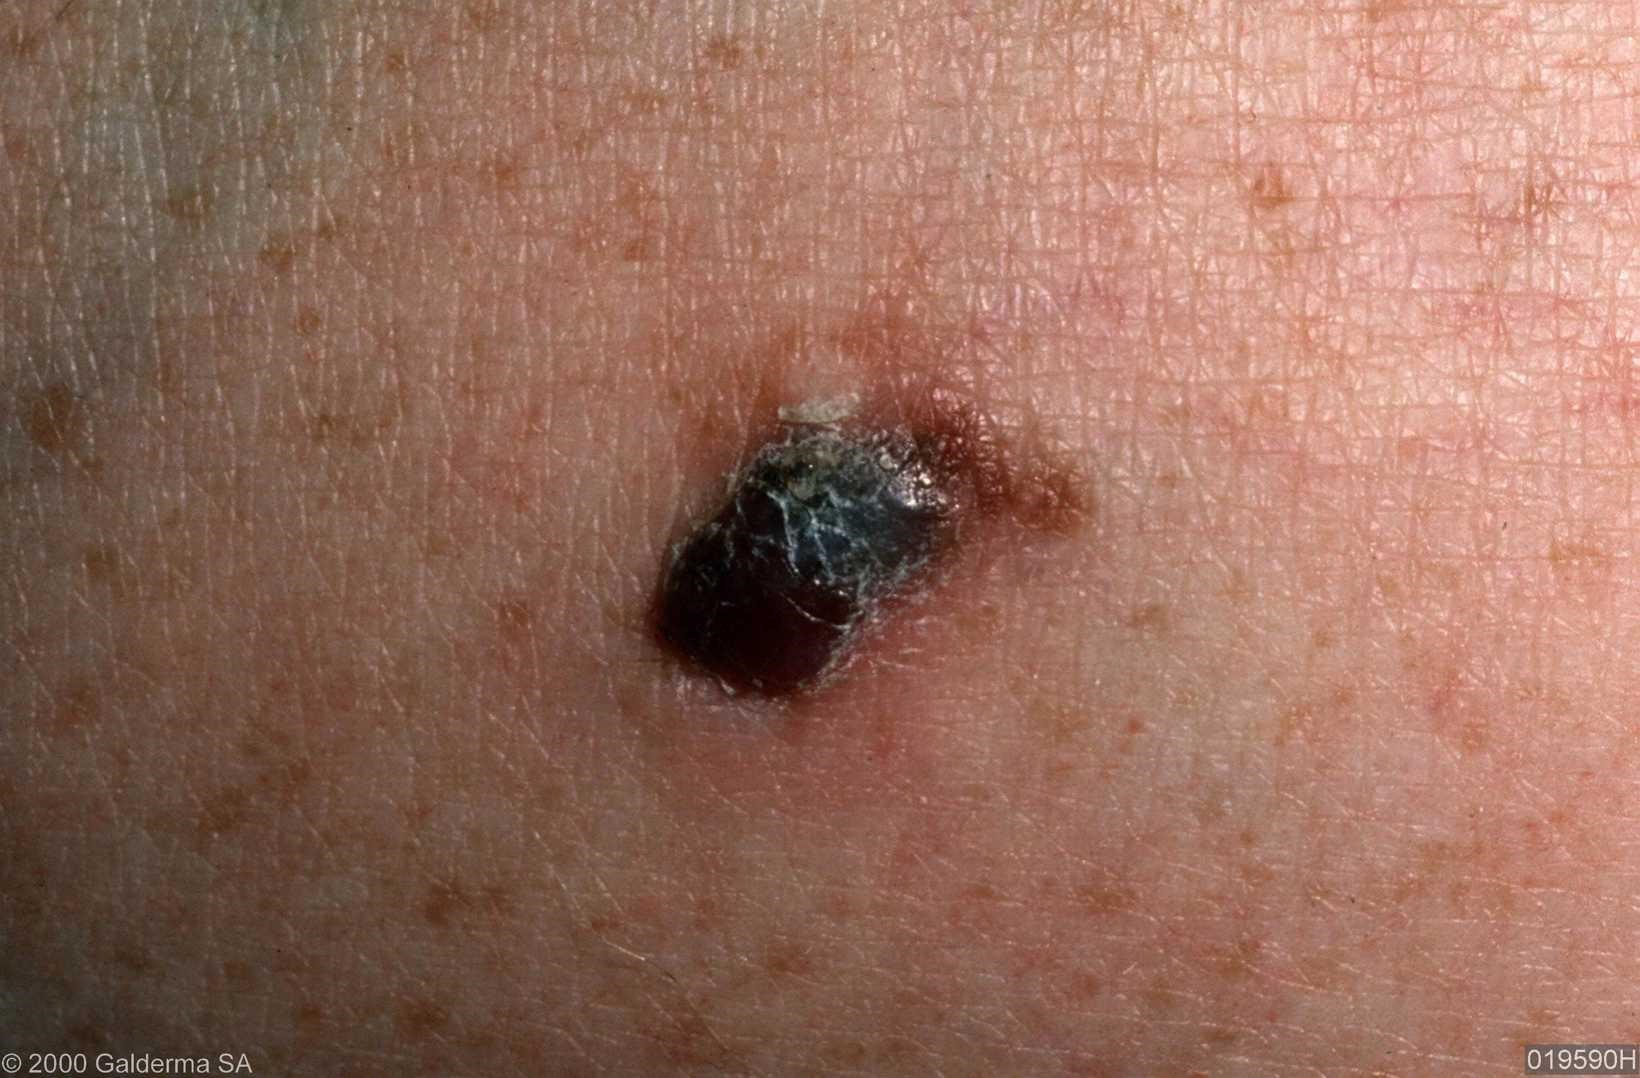
\includegraphics[width=0.45\textwidth]{images/sd260_mel.jpg}} &
		\subcaptionbox{\centering Melanocytic \mbox{Nevus}}{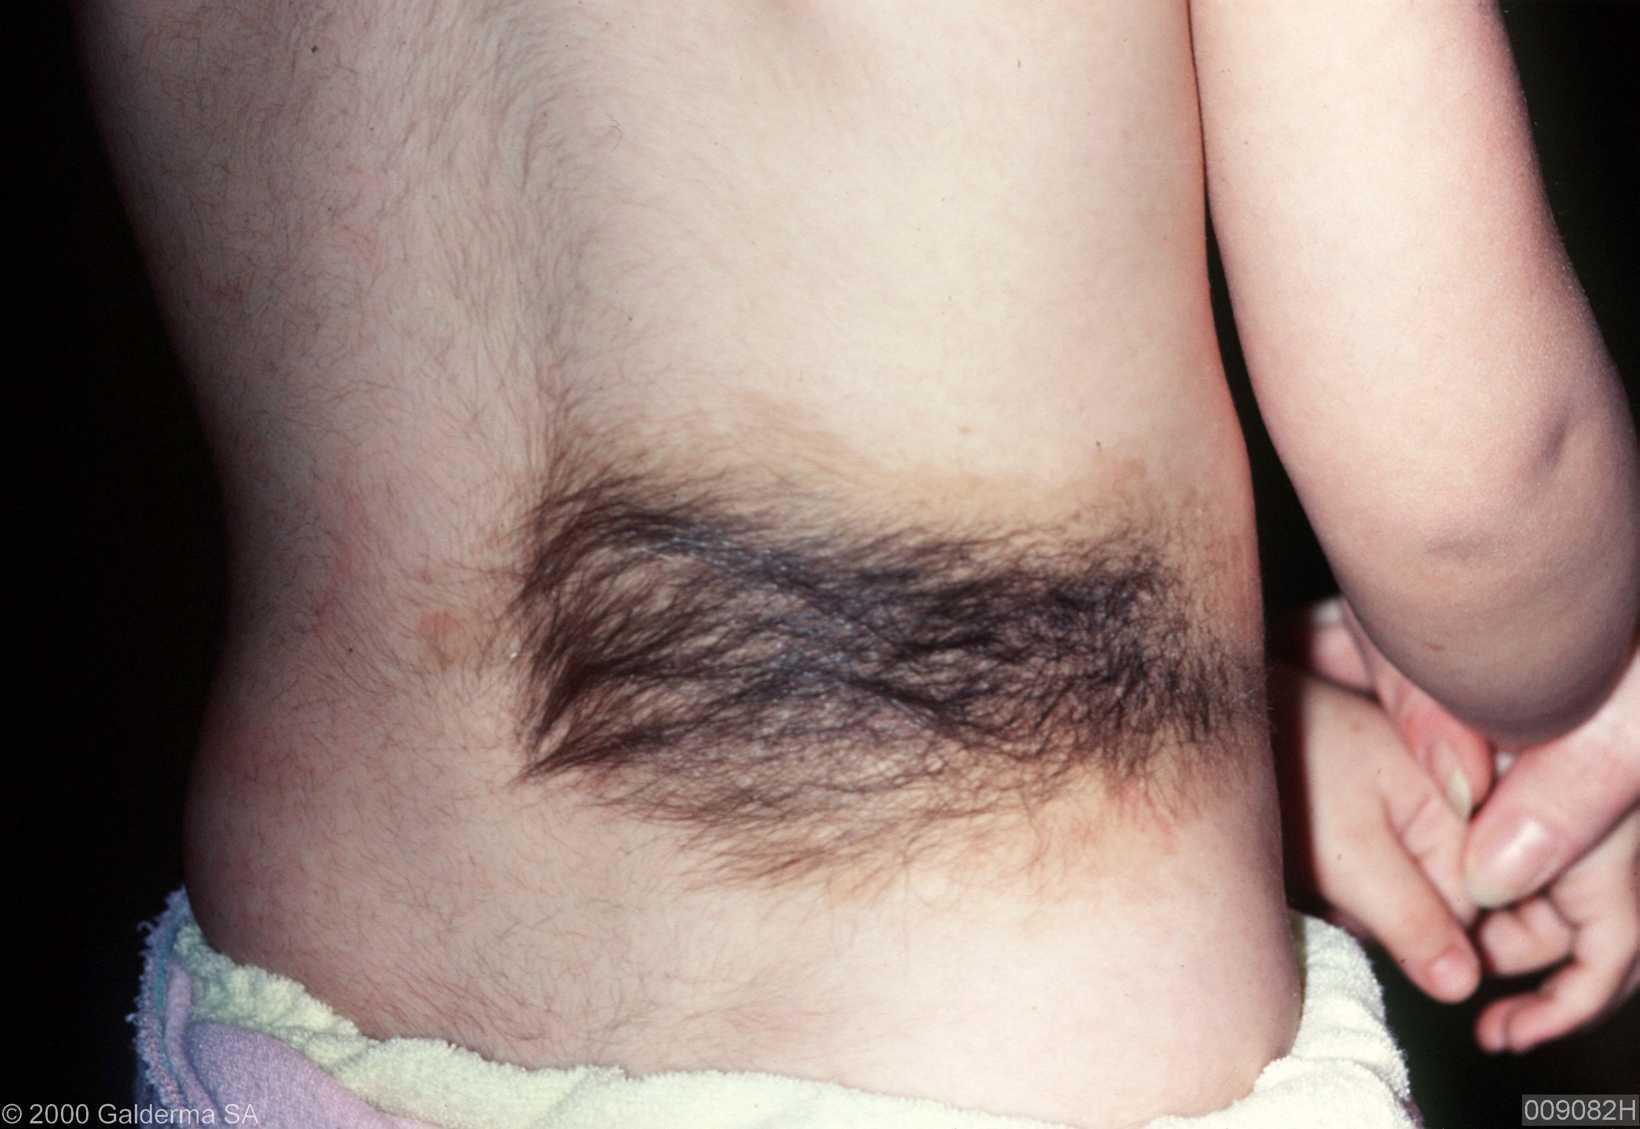
\includegraphics[width=0.45\textwidth]{images/sd260_nv.jpg}} \\
		\subcaptionbox{\centering Basal Cell \mbox{Carcinoma}}{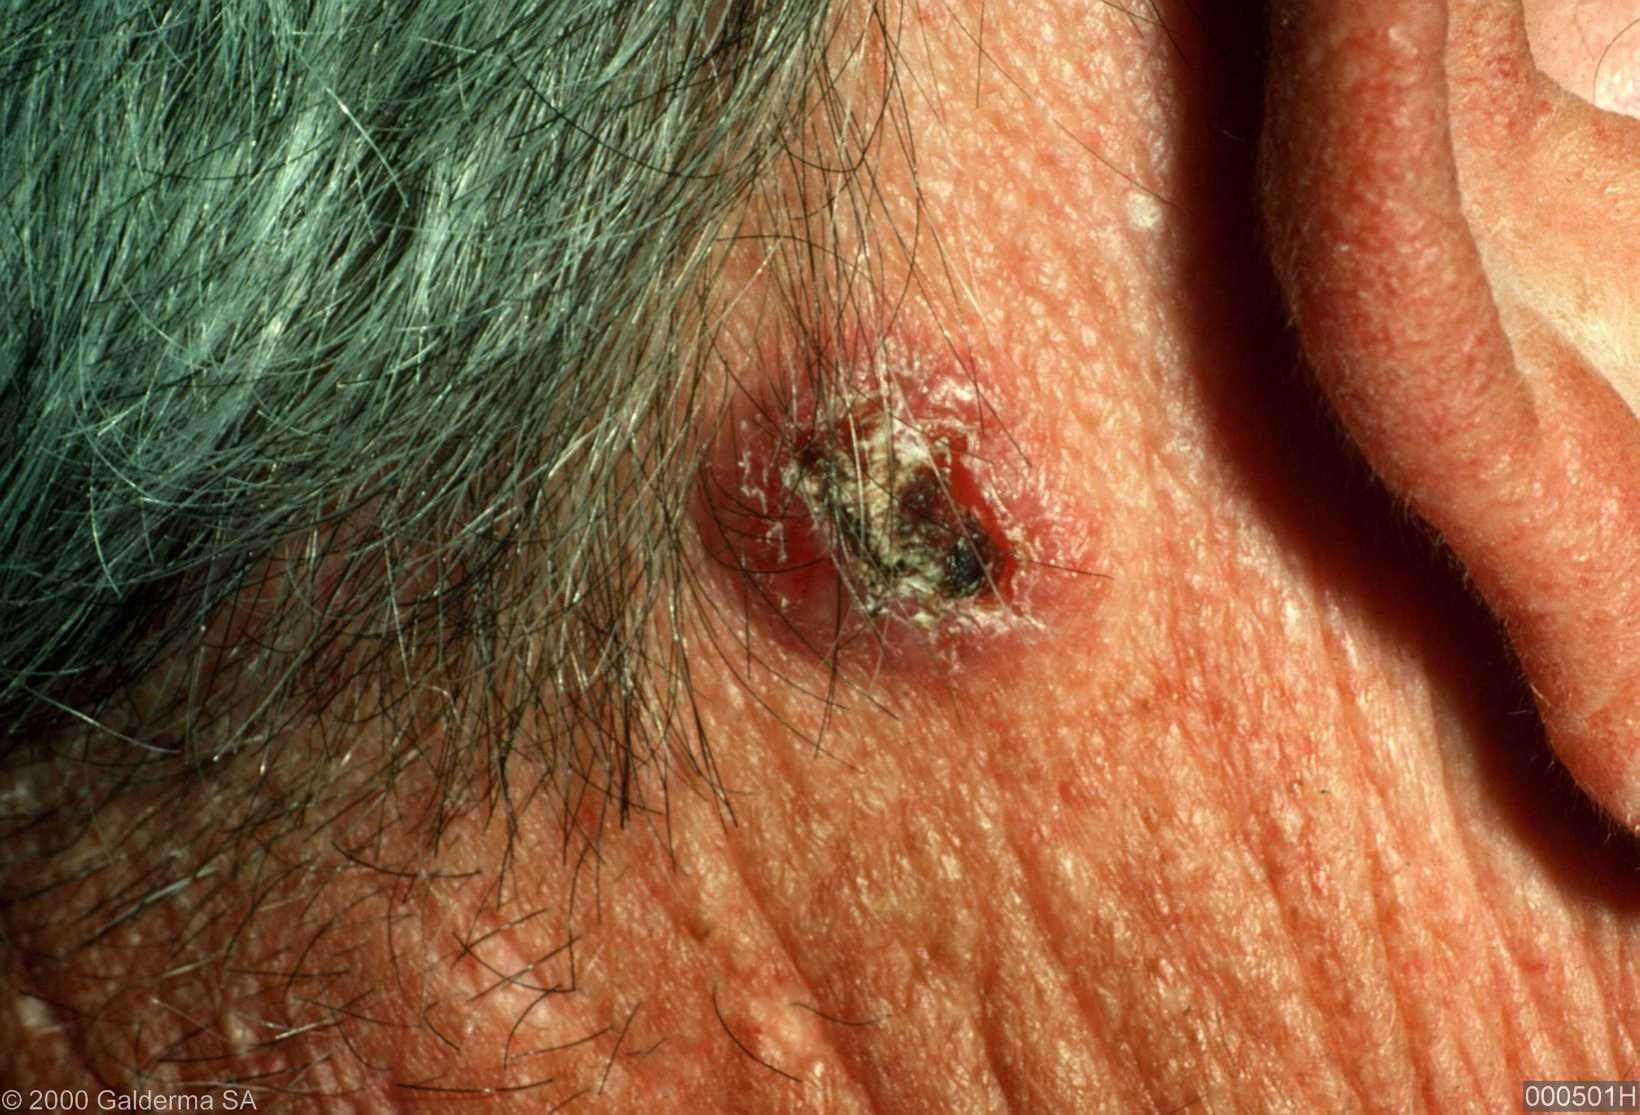
\includegraphics[width=0.45\textwidth]{images/sd260_bcc.jpg}} &
		\subcaptionbox{\centering Actinic Keratosis}{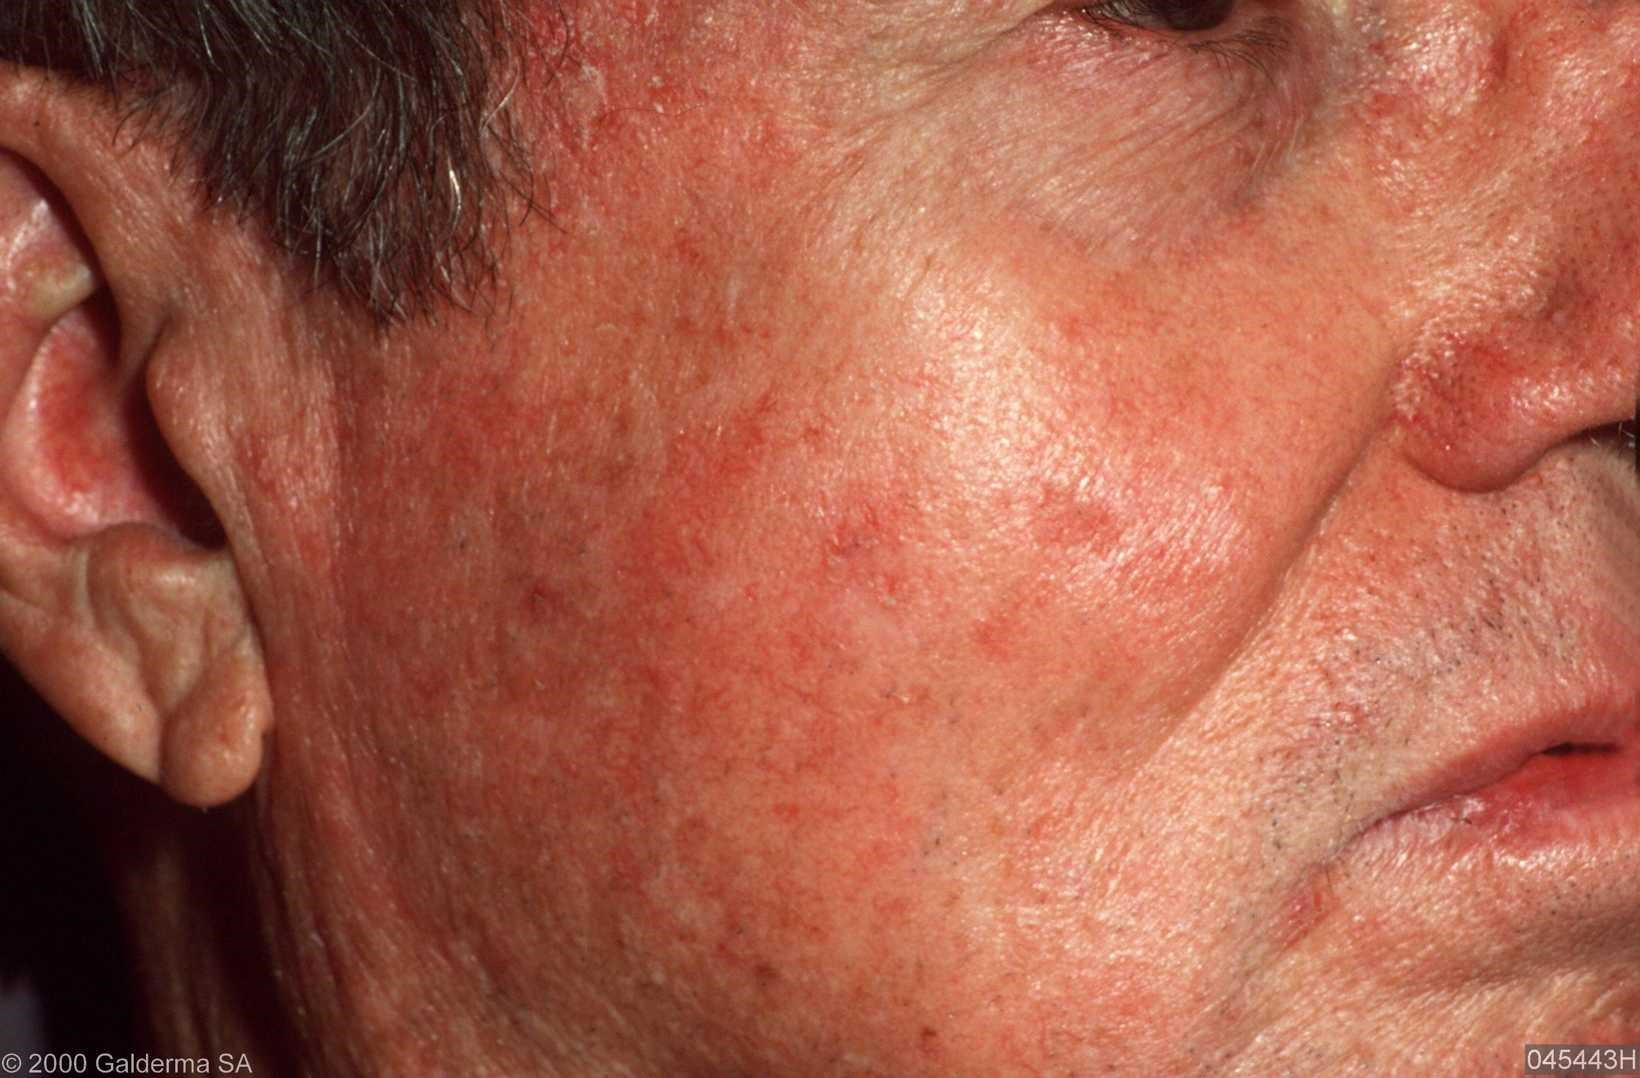
\includegraphics[width=0.45\textwidth]{images/sd260_ak.jpg}} \\
		\subcaptionbox{\centering Benign Keratosis}{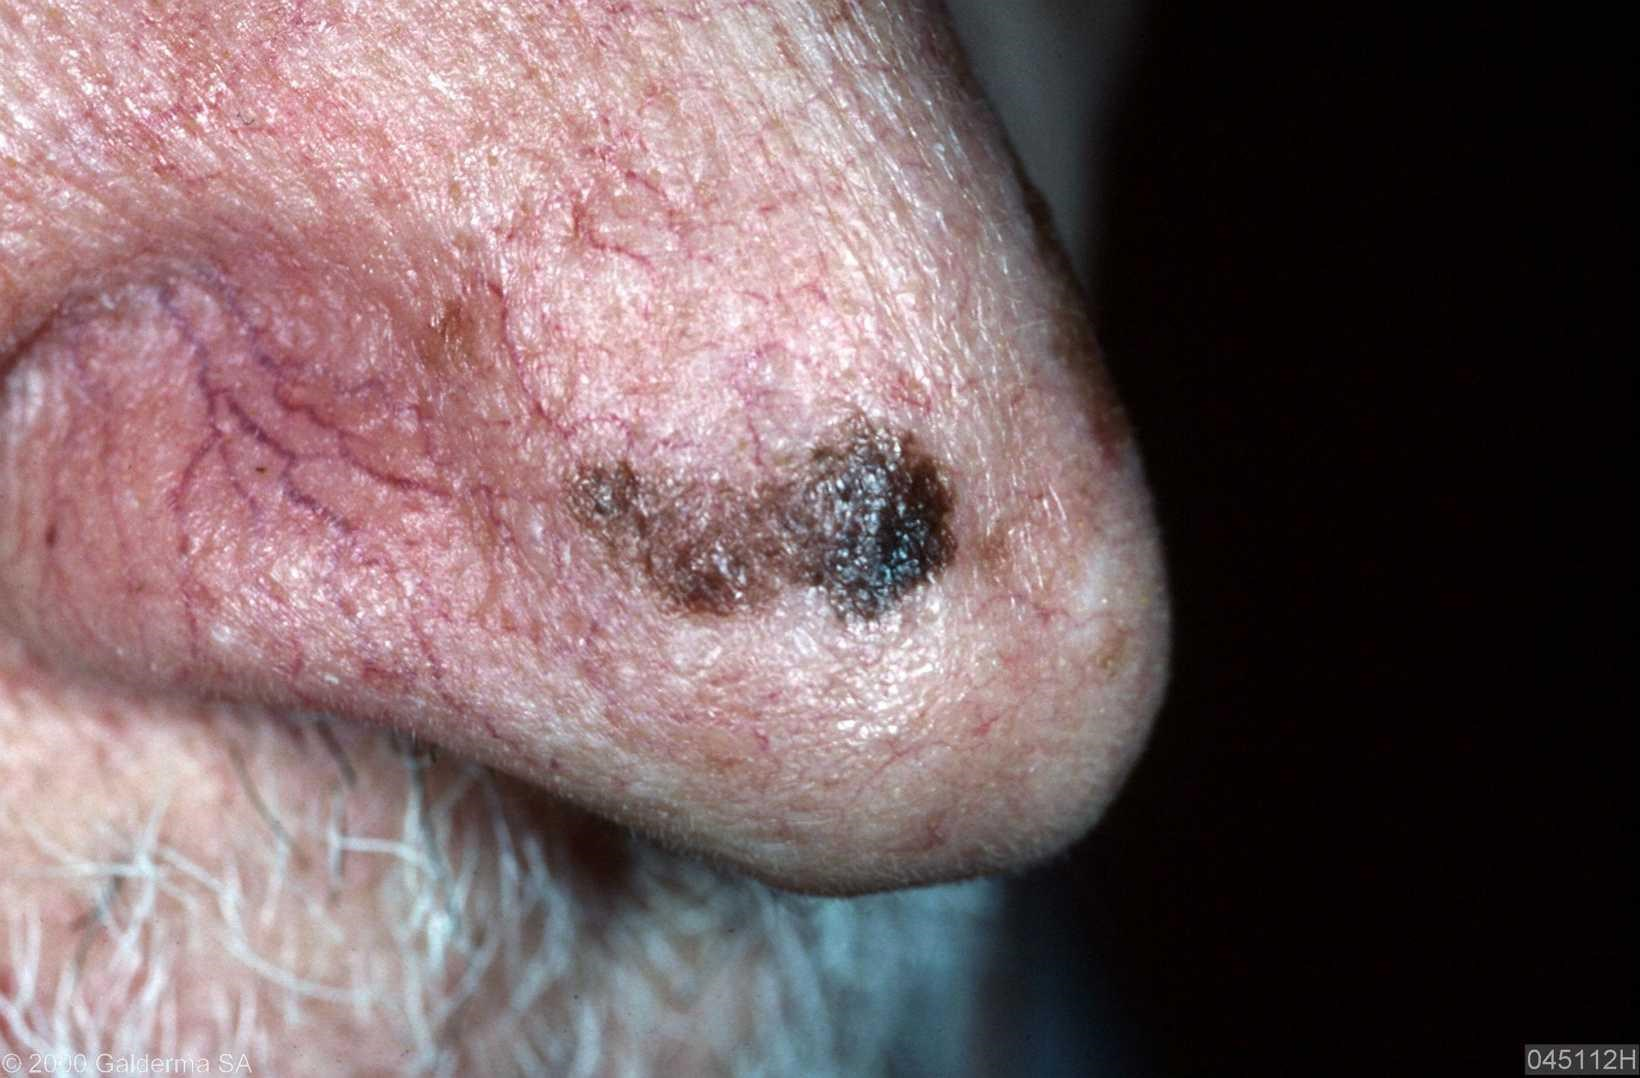
\includegraphics[width=0.45\textwidth]{images/sd260_bkl.jpg}} &
		\subcaptionbox{\centering Dermatofibroma}{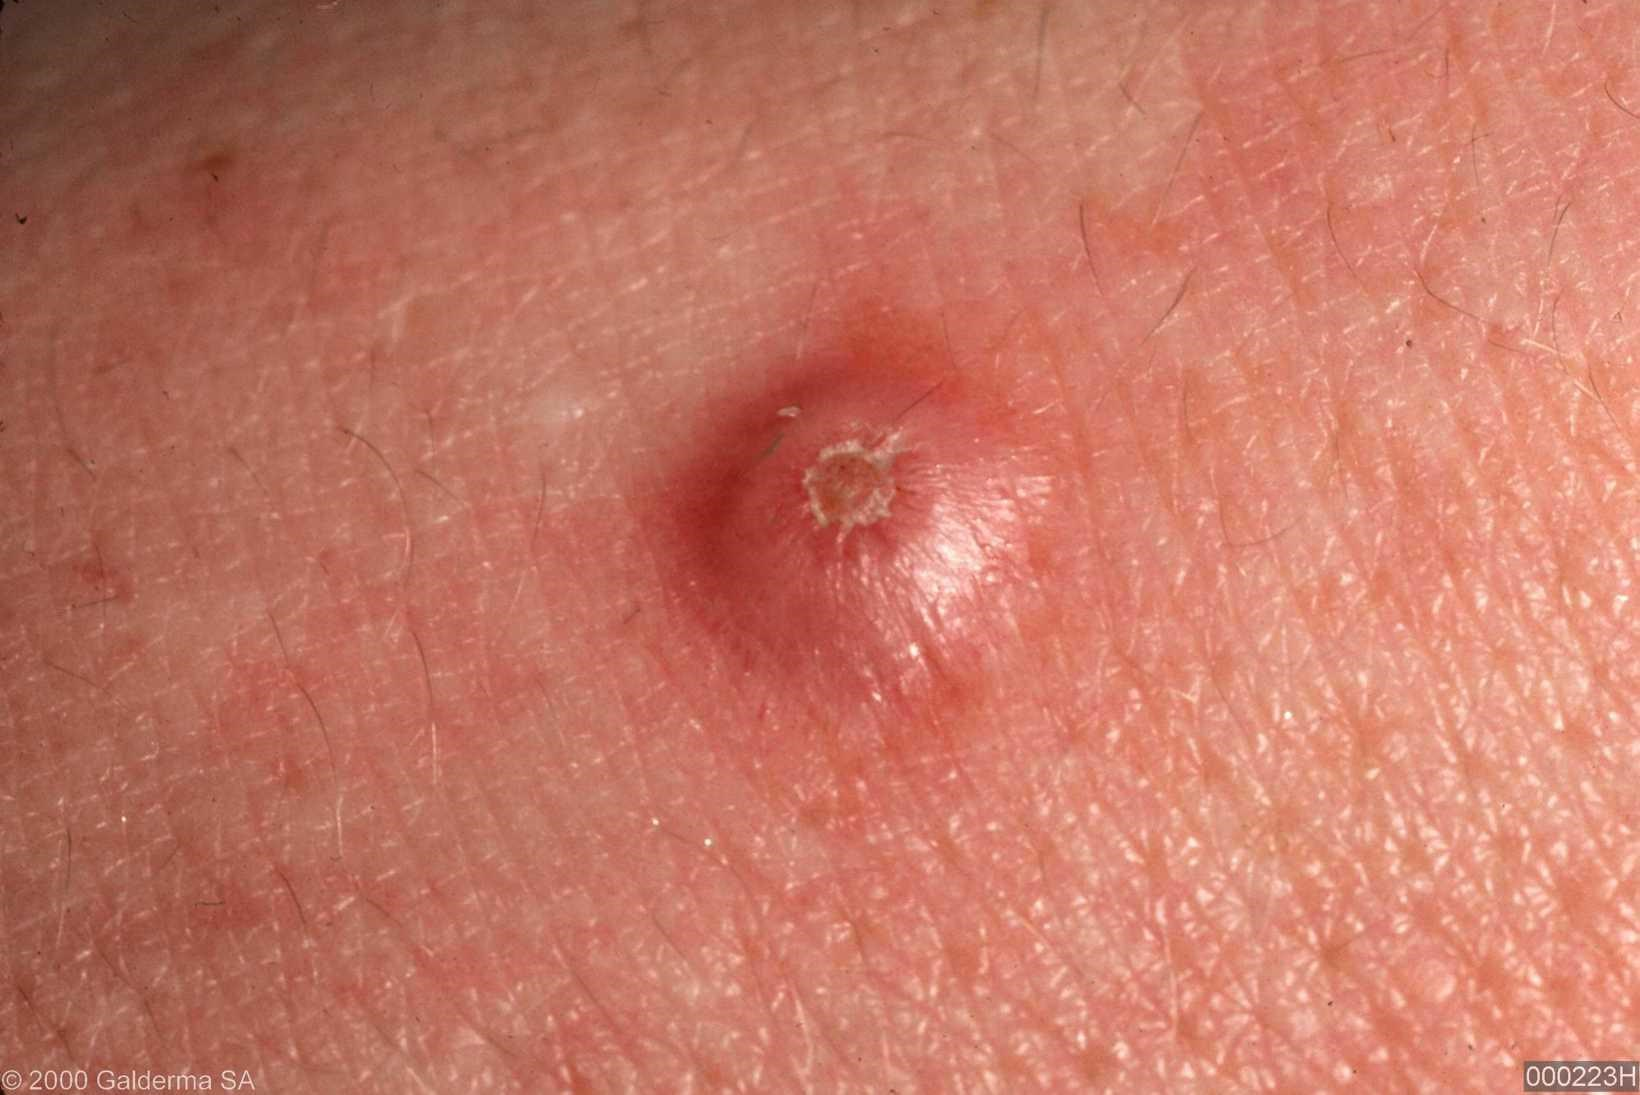
\includegraphics[width=0.45\textwidth]{images/sd260_df.jpg}} \\
		\multicolumn{2}{c}{\subcaptionbox{\centering Squamous Cell \mbox{Carcinoma}}{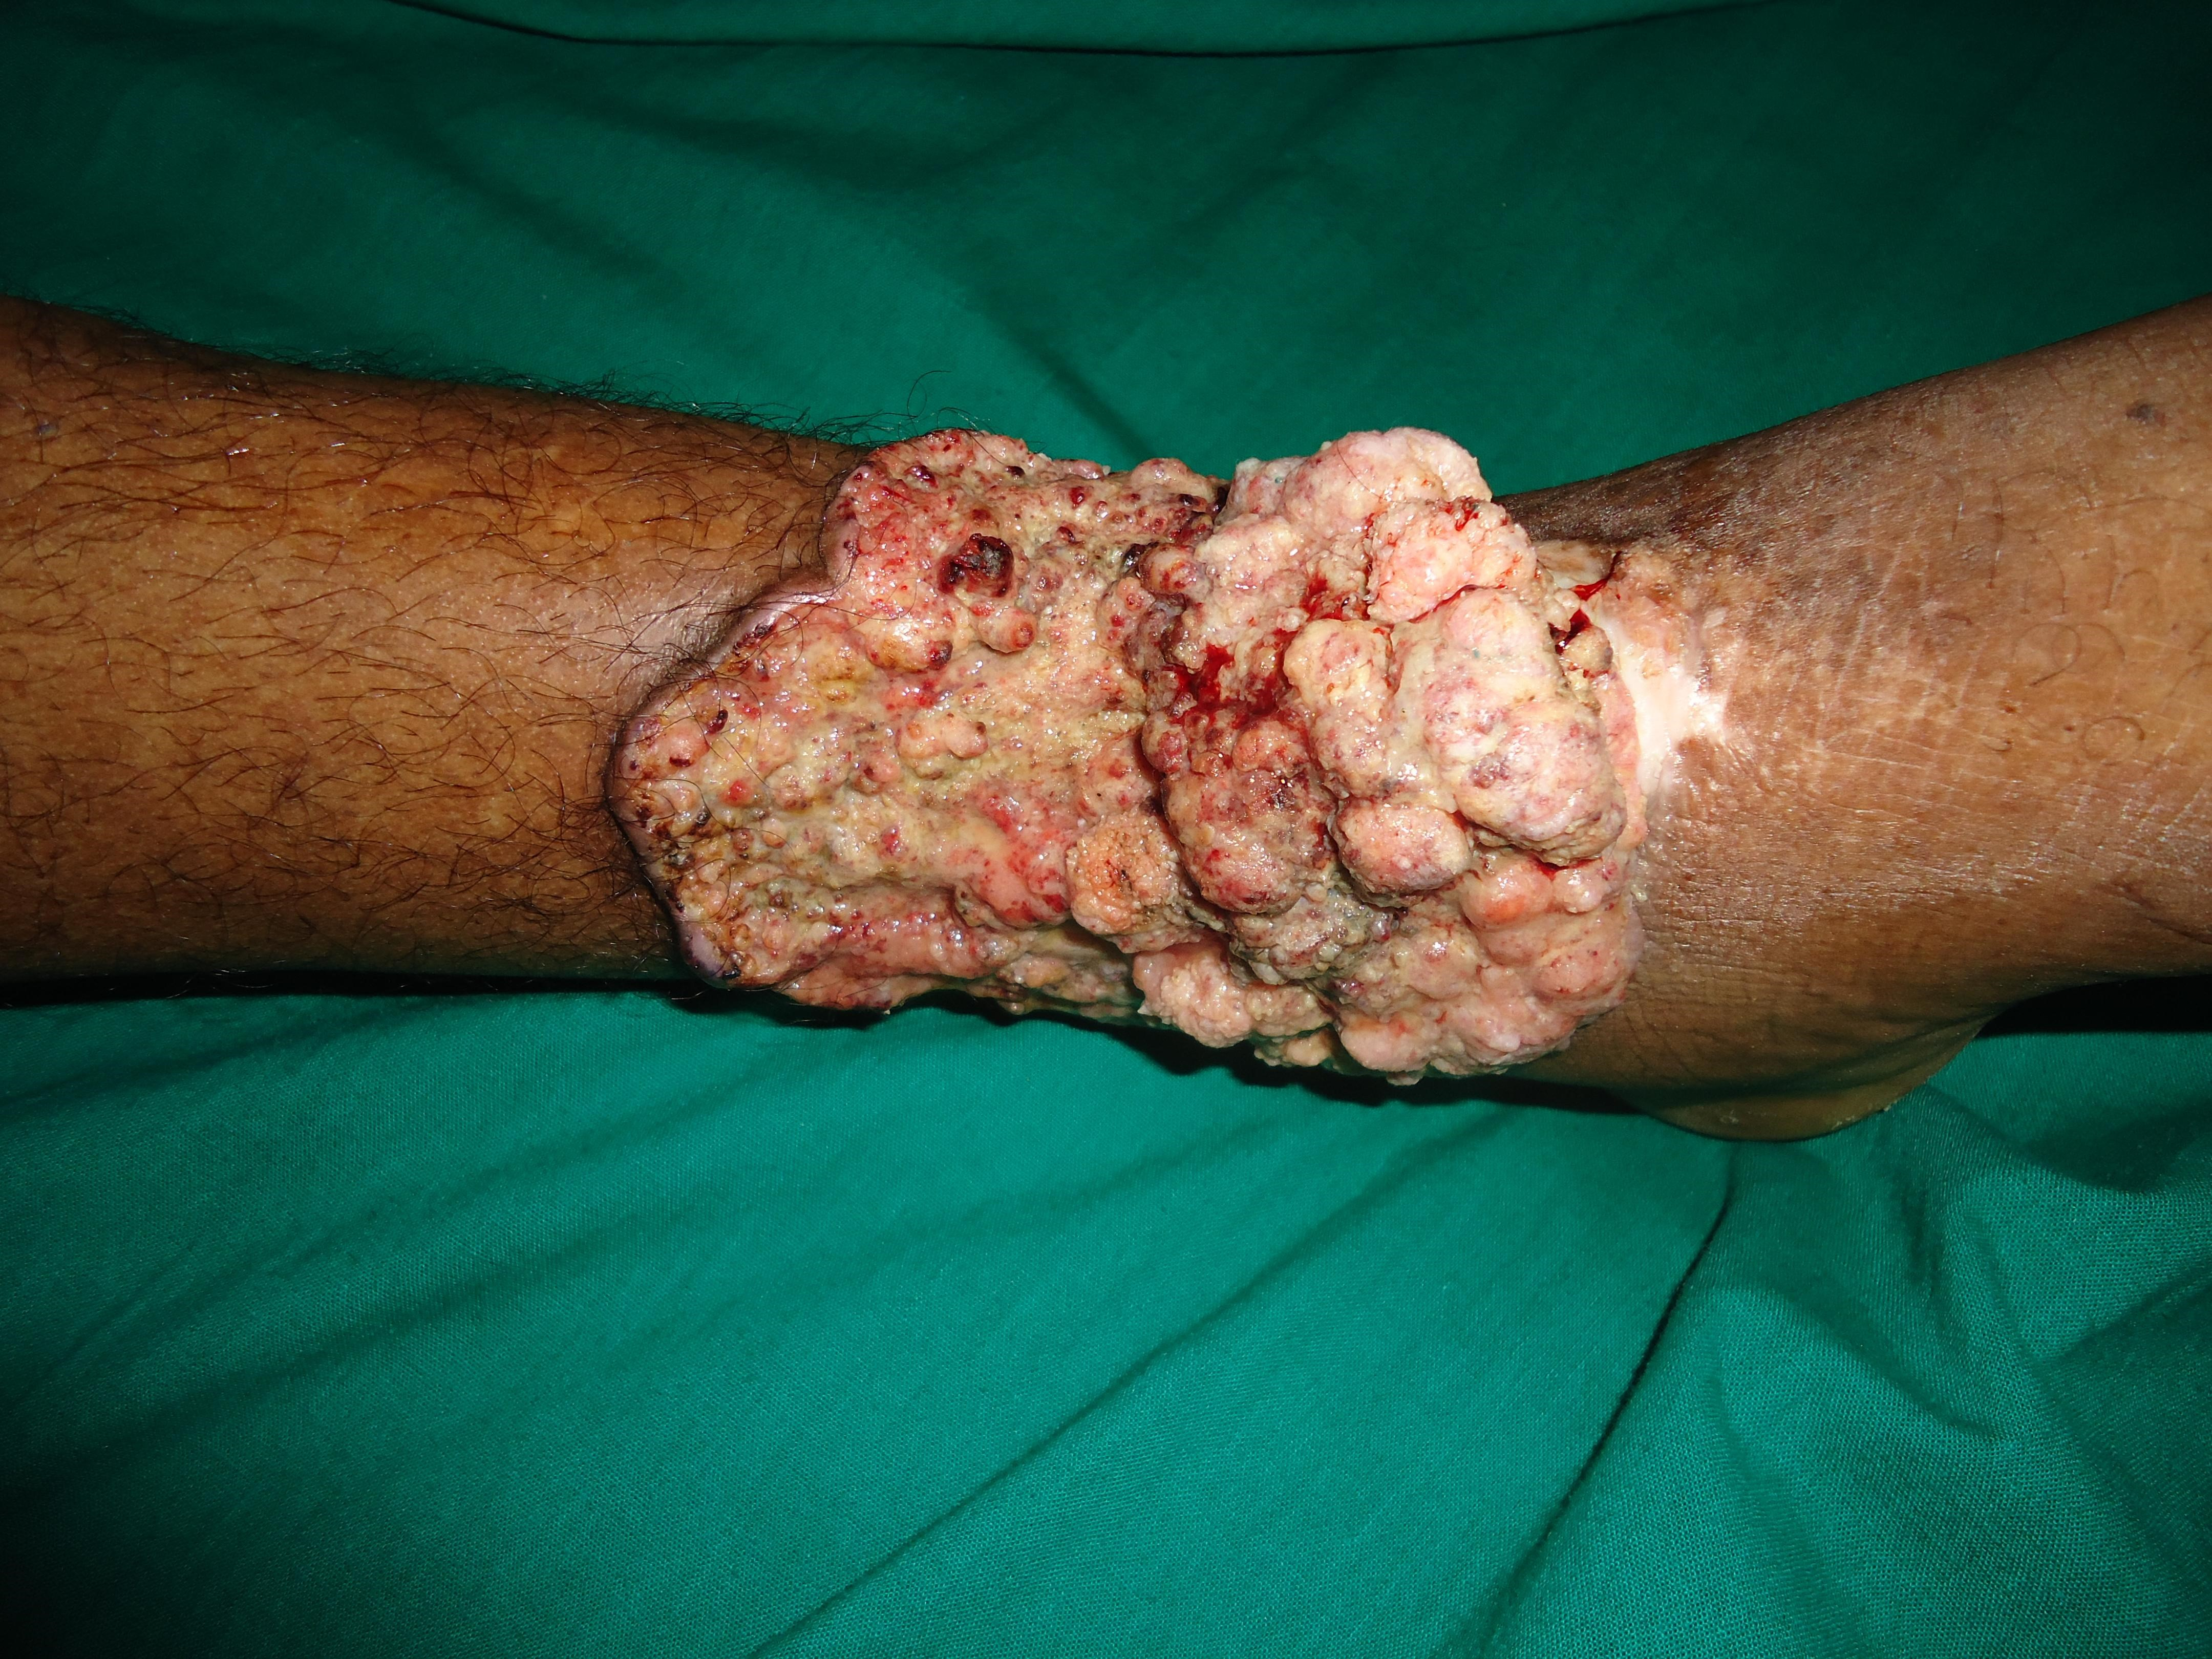
\includegraphics[width=0.45\textwidth]{images/sd260_scc.jpg}}}
	\end{tabular}
	\caption{Example images from the SD-260 dataset~\citep{yang2019self}.}
	\label{fig:sd260_examples}
\end{figure}

To facilitate deep learning experiments, the four skin lesion datasets used in this study were intentionally restricted to a set of seven diagnostic categories. The specific seven categories were chosen based on their representation across the four datasets. For example, vascular lesions were excluded from the ISIC 2019 dataset, and classes such as angioma and solar lentigo were excluded from the Tayside dataset because they were not well represented in the other two datasets. The ISIC 2019, SD-260, Tayside, and Forth Valley data subsets used in the study contained 25078, 13814, 2218, and 1518 images, respectively (Table~\ref{tab:generalisation_datasets}).

\begin{table}[h]
	\centering
	\caption{Number of images per diagnosis in each dataset.}
	\label{tab:generalisation_datasets}
	\resizebox{\textwidth}{!}{%
		\begin{tabular}{|ll|l|l|l|l|}
			\hline
			&                             & \textbf{ISIC 2019} & \textbf{SD-260} & \textbf{Tayside} & \textbf{Forth Valley} \\ \hline
			\multicolumn{1}{|l|}{\textbf{Benign}} & Actinic keratosis (B52)     & 867                & 1434            & 414              & 144                   \\
			\multicolumn{1}{|l|}{}                & Dermatofibroma (X9002)      & 239                & 303             & 56               & 78                    \\
			\multicolumn{1}{|l|}{}                & Naevus, melanocytic (X31z)  & 12875              & 1401            & 577              & 531                   \\
			\multicolumn{1}{|l|}{}                & Seborrhoeic keratosis (X01) & 2624               & 1133            & 538              & 290                   \\ \hline
			\multicolumn{1}{|l|}{\textbf{Malignant}} &
			\begin{tabular}[c]{@{}l@{}}Melanoma (X41) / \\ Melanoma in situ (X40)\end{tabular} &
			4522 &
			7094 &
			78 &
			205 \\
			\multicolumn{1}{|l|}{} &
			\begin{tabular}[c]{@{}l@{}}Squamous cell carcinoma (X12) / \\ Squamous cell carcinoma in situ (X11)\end{tabular} &
			628 &
			17 &
			176 &
			91 \\
			\multicolumn{1}{|l|}{}                & Basal cell carcinoma (X20)  & 3323               & 2432            & 379              & 179                   \\ \hline
			\textit{\textbf{Total}}               & \textit{}                   & \textit{25078}     & \textit{13814}  & \textit{2218}    & \textit{1518}         \\ \hline
		\end{tabular}%
	}
\end{table}

\subsection{Training Parameters}
\label{subsec:generalisation_training}
In this study, we employed two methods for image classification using deep learning. The first method was a convolutional neural network, specifically an EfficientNet architecture~\citep{tan2019efficient} with a compound coefficient of 7 and an additional fully connected layer of 512 neurons preceding the output layer. The second method was a SWIN-B transformer~\citep{liu2021swin}, a state-of-the-art visual transformer network for image classification.

Subsequent training sessions were conducted for 40 epochs, with the model being saved each time the lowest validation loss was achieved. The weights were optimized using stochastic gradient descent with batches of 16 images and a triangular$^2$ cyclical scheduler~\citep{smith2017cyclical}, which alternated the learning rate between $10^{-5}$ and $10^{-2}$ and the momentum between 0.8 and 0.9. All images were pre-processed by cropping, resizing to 224 x 224 pixels, and normalizing the pixel values between 0.0 and 1.0. Data augmentation was used to improve generalization, specifically using a range of geometric and photometric transformations applied randomly when sampled.

Given an image, the deep network models predicted class probabilities for each of the seven diagnostic classes. These probabilities were constrained, by definition, to sum to one. Three of the seven classes represented malignant lesions. By summing the probabilities of these three classes, the probability that the observed lesion is malignant, assuming the class probabilities computed were well-calibrated (Chapter \ref{ch:classification_claibration}). This was used to evaluate the ability of the CNN and SWIN transformer models to identify malignant lesions. Specifically, ROC curves were used to quantify the sensitivity-specificity trade-offs that can be obtained on the macroscopic image datasets. 

\subsection{Experiment Setup}
\label{subsec:generalisation_experiment}
The ability of the models to classify lesion images from each dataset was first evaluated after training on images from that same dataset. When utilizing the larger datasets, ISIC 2019 and SD-260, a disjoint split of 60\% for training, 20\% for validation, and 20\% for testing was employed. These splits were static, and all training and testing with the datasets utilized the same splits. In contrast, given the limited size of the Tayside and Forth Valley datasets, 10-fold cross-validation was utilized to estimate performance, with each fold containing disjoint training (70\%), validation (20\%), and test (10\%) sets. These splits were also static across each fold, with the performance being estimated by averaging the 10 test results.

Subsequently, cross-dataset performance was evaluated by measuring the class-balanced accuracy of each model when tested on data from datasets not used for training the model. Deep classifiers pre-trained with ImageNet~\citep{deng2009imagenet} were trained on data from each of the datasets and then tested on each of the datasets. The composition of the training sets was identical to those used in the internal data classification experiment.

Finally, the effect of transfer learning between the dermatology datasets using CNN and SWIM transformer models was evaluated. It is noted that all models in the experiments were pre-trained on ImageNet. Further pre-training was then performed on dermatology datasets. The effect of transfer between the large ISIC 2019 and SD-260 datasets was evaluated first. Secondly, the effect of transfer when the target domains (test data) were Tayside and Forth Valley data was investigated, utilizing multi-dataset pre-training sequences, such as pre-training on SD-260 data and then training on Forth Valley training data, denoted “SD-260, Forth Valley” or pre-training on ISIC 2019 data, then on SD-260 data, and finally on Tayside training data, denoted “ISIC 2019, SD-260, Tayside”.


\subsection{Results}
\label{subsec:generalisation_results}
Table~\ref{tab:generalisation_results} presents the balanced class accuracies obtained using CNN and SWIN transformer models when trained and tested on data from the four datasets. The diagonal entries, in bold, reflect the internal accuracies obtained when disjoint test and training sets from the same source dataset were used. The SWIN transformer achieved 98\% on each of the large public domain datasets, ISIC 2019 and SD-260. Accuracies on the smaller macroscopic NHS datasets were lower, as anticipated, with the SWIN transformer achieving 90.2\% and 87.5\% on Forth Valley and Tayside data, respectively.

\begin{table}[h]
	\centering
	\caption{Class-balanced accuracy when training and testing on the various datasets.}
	\label{tab:generalisation_results}
	\resizebox{\textwidth}{!}{%
		\begin{tabular}{|l|l|l|l|l|l|}
			\hline
			& Training Data & ISIC 2019      & SD-260         & Tayside        & Forth Valley   \\ \hline
			\textbf{CNN}  & ISIC 2019     & \textbf{0.978} & 0.804          & 0.825          & 0.855          \\
			& SD-260        & 0.879          & \textbf{0.969} & 0.855          & 0.867          \\
			& Tayside       &                &                & \textbf{0.875} & 0.850          \\
			& Forth Valley  &                &                & 0.847          & \textbf{0.891} \\ \hline
			\textbf{SWIN} & ISIC 2019     & \textbf{0.979} & 0.813          & 0.825          & 0.868          \\
			& SD-260        & 0.870          & \textbf{0.980} & 0.867          & 0.878          \\
			& Tayside       &                &                & \textbf{0.875} & 0.859          \\
			& Forth Valley  &                &                & 0.849          & \textbf{0.902} \\ \hline
		\end{tabular}%
	}
\end{table}

Overall, in the absence of training data from the target domains, training on SD-260 data provided the best test accuracies on all test datasets. Models trained on ISIC data did not generalize well to the other datasets, while models trained on SD-260 data generalized slightly better but still poorly. Generalization between the Tayside and Forth Valley datasets was better, with relatively small drops in test accuracy. Models trained on Tayside data achieved test results on Forth Valley data only 1.6\% and 2.5\% lower than test results on Tayside data.

Additionally, it was observed that models trained and tested on ISIC data did not benefit from pre-training on SD-260; ISIC test results with SD-260 pre-training were 97.7\% and 97.1\% for CNN and SWIN, respectively. Similarly, models trained and tested on SD-260 data did not benefit from pre-training on ISIC data. SD-260 test results with ISIC pre-training were 96.7\% and 97.7\% for CNN and SWIN, respectively.

Table~\ref{tab:generalisation_models} reports balanced class accuracies when CNN and SWIN transformers were tested on Tayside and Forth Valley data after various multi-dataset training sequences. In each case, pre-training on SD-260 data followed by fine-tuning on data from the target domain was found to be effective.


\begin{table}[h]
	\centering
	\caption{Balanced class accuracy when CNN and SWIN transformers are tested on Tayside and Forth Valley data after various multi-dataset training sequences. }
	\label{tab:generalisation_models}
	\resizebox{\textwidth}{!}{%
		\begin{tabular}{|l|l|l|l|}
			\hline
			& Training Datasets               & Tayside        & Forth Valley   \\ \hline
			CNN  & SD-260, ISIC 2019               & 0.832          & 0.860          \\
			& ISIC 2019, SD-260               & 0.850          & 0.868          \\
			& ISIC 2019, Tayside              & 0.880          & 0.875          \\
			& SD-260, Tayside                 & \textbf{0.890} & 0.870          \\
			& ISIC 2019, SD-260, Tayside      & 0.879          & 0.876          \\
			& ISIC 2019, Forth Valley         & 0.850          & 0.900          \\
			& SD-260, Forth Valley            & 0.861          & \textbf{0.907} \\
			& ISIC 2019, SD-260, Forth Valley & 0.852          & 0.904          \\ \hline
			SWIN & SD-260, ISIC 2019               & 0.830          & 0.868          \\
			& ISIC 2019, SD-260               & 0.863          & 0.877          \\
			& ISIC 2019, Tayside              & 0.881          & 0.884          \\
			& SD-260, Tayside                 & \textbf{0.891} & 0.891          \\
			& ISIC 2019, SD-260, Tayside      & 0.890          & 0.896          \\
			& ISIC 2019, Forth Valley         & 0.854          & 0.910          \\
			& SD-260, Forth Valley            & 0.867          & 0.914          \\
			& ISIC 2019, SD-260, Forth Valley & 0.859          & \textbf{0.916} \\ \hline
		\end{tabular}%
	}
\end{table}

The results are also illustrated in Figure~\ref{fig:generalisation_models} which shows how test accuracies changed when different datasets were used for training and transfer learning. It was observed that training only on the large ISIC and SD-260 datasets gave relatively poor results, while training on a small dataset from the target domain, after pre-training only on ImageNet, performed better. The most accurate models were obtained by pre-training on the large dermatology datasets followed by further training on data from the target domain.

\begin{figure}[!h]
	\centering
	\captionsetup[subfigure]{singlelinecheck=false}
	\begin{tabular}{c}
		\subcaptionbox{\centering Testing on the Tayside dataset.}{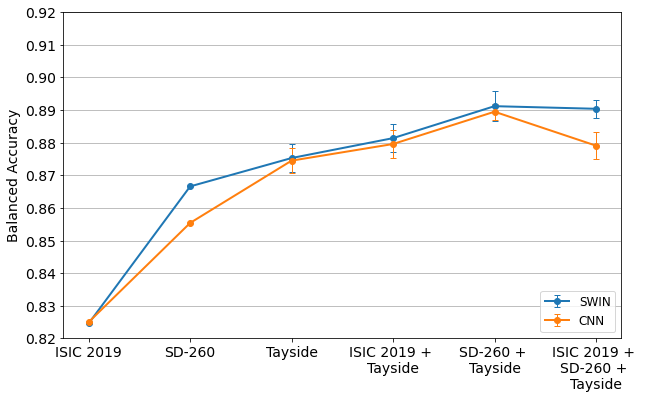
\includegraphics[width=0.9\textwidth]{images/tayside_model.png}} \\
		\subcaptionbox{\centering Testing on the Forth Valley dataset.}{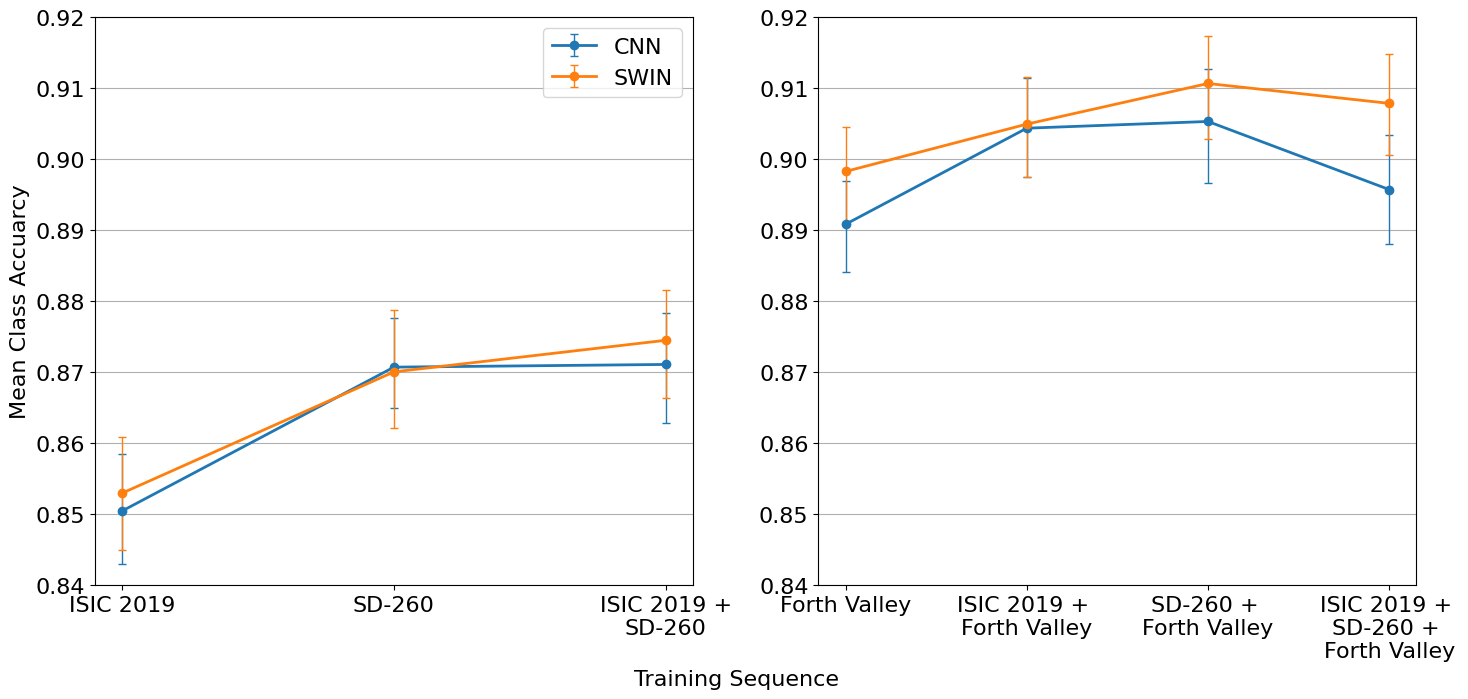
\includegraphics[width=0.9\textwidth]{images/forth_valley_model.png}}
	\end{tabular}
	\caption{Balanced accuracy of models when tested on Tayside and Forth Valley datasets after various pre-training sequences. Bars are +/- one standard error computed from the variance over cross-validation folds.}
	\label{fig:generalisation_models}
\end{figure}

Figure~\ref{fig:generalisation_testing} illustrates the extent to which models trained for the Tayside domain were able to generalize to the Forth Valley domain, and vice-versa. The solid curves plot the accuracies obtained when training on data from the test domain, with and without pre-training on the large public domain datasets. Dashed curves plot accuracies when training on data from the other test domain. The drops in accuracy when generalizing between Tayside and Forth Valley dataset were 2-3\% using the SWIN transformer model.

\begin{figure}[!h]
	\centering
	\captionsetup[subfigure]{singlelinecheck=false}
	\begin{tabular}{c}
		\subcaptionbox{\centering Testing on the Tayside dataset.}{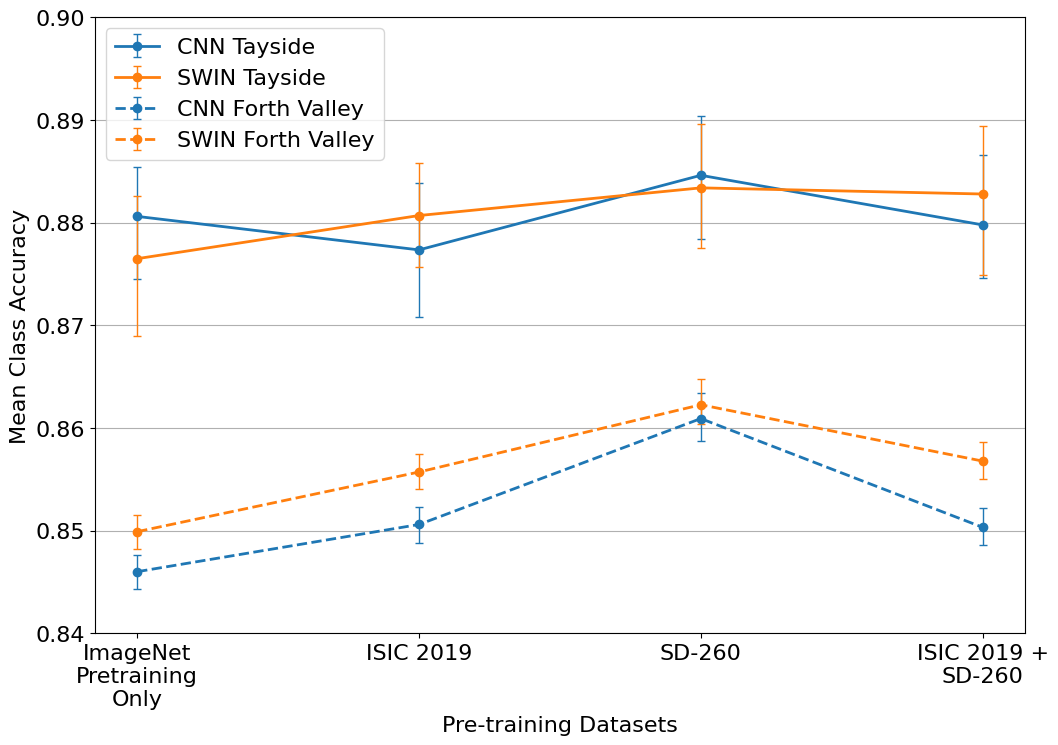
\includegraphics[width=0.9\textwidth]{images/tayside_testing.png}} \\
		\subcaptionbox{\centering Testing on the Forth Valley dataset.}{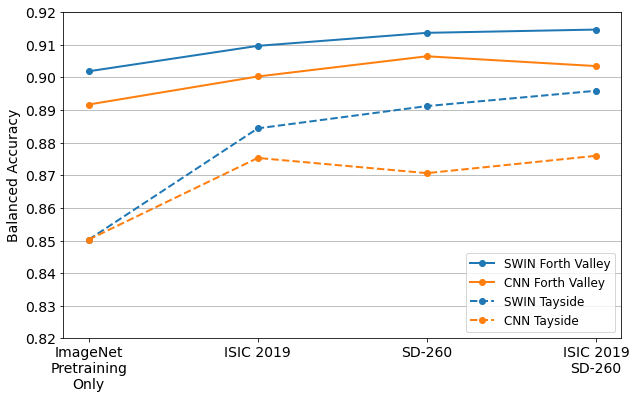
\includegraphics[width=0.9\textwidth]{images/forth_valley_testing.png}}
	\end{tabular}
	\caption{Balanced accuracy of the models demonstrating the performance of dataset cross-generalisation between the Tayside and Forth Valley datasets.}
	\label{fig:generalisation_testing}
\end{figure}

Finally, binary classification performance in the form of ROC curves is reported in Figure~\ref{fig:generalisation_roc}. These curves were generated using models pre-trained on SD-260 prior to training on either Tayside or Forth Valley data. It was observed that the Forth Valley curves dominated the Tayside curves, and curves for models trained on the test domain dominated curves trained on the other domain.

\begin{figure}[!h]
	\centering
	\captionsetup[subfigure]{singlelinecheck=false}
	\begin{tabular}{c}
		\subcaptionbox{\centering Testing on the Tayside dataset.}{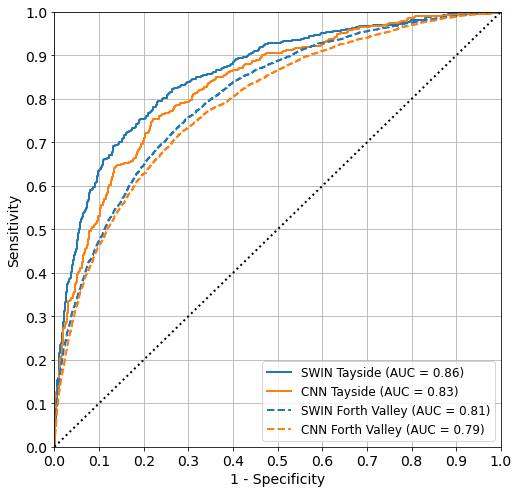
\includegraphics[width=0.85\textwidth]{images/tayside_roc.png}} \\
		\subcaptionbox{\centering Testing on the Forth Valley dataset.}{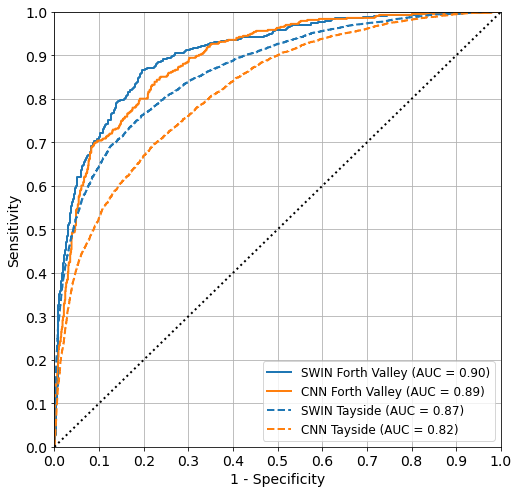
\includegraphics[width=0.85\textwidth]{images/forth_valley_roc.png}}
	\end{tabular}
	\caption{ROC curves for CNNs and SWIN transformers pre-trained on SD-260 prior to training on either Tayside or Forth Valley data.}
	\label{fig:generalisation_roc}
\end{figure}



\section{Conclusion}
\label{sec:generalisation_conclusion}
It is well-established that deep learning classifiers benefit from large training sets. However, it is also known that test performance is negatively affected by variations in image acquisition, image quality, and the population being imaged. This presents challenges in the development of dermatology diagnostic systems that can be deployed in multiple sites, as such conditions can vary geographically and over time. Curation of large datasets can be costly at a local level, yet learning systems need to be attuned to local conditions.

Our results suggest that the SWIN transformer should be preferred over the EfficientNet convolutional neural network. The transformer obtained accuracies of 98\% on both ISIC 2019 and SD-260 test datasets, provided it was trained on data from the same domain. However, cross-domain generalization (training on ISIC 2019 and testing on SD-260) led to a weaker 81\% accuracy. Training on SD-260 and testing on ISIC 2019 yielded a better 88\% accuracy, possibly due to the more varied nature of the SD-260 dataset (Table~\ref{tab:generalisation_results}).

The ISIC 2019 and SD-260 datasets are relatively large, though still not comparable to datasets used for deep learning in computer vision. The focus of our study was how to obtain good performance on challenging local data with limited availability of diagnostic labels. The two NHS datasets used to explore this question were sourced from Tayside and Forth Valley, the latter having images of more consistent and higher quality than the former. Transformers yielded accuracies of 87.5\% and 90.2\%, respectively, when trained and tested on data from these domains. This was better than results obtained by training on the larger SD-260 and ISIC 2019 datasets (Figure~\ref{fig:generalisation_models}), highlighting the benefit of training with data from the local target domain. We found that by pre-training on SD-260 and then on data from the local target domain, further increases to 89.1\% and 91.4\% were obtained (Figure~\ref{fig:generalisation_testing}, solid blue lines).

Given their geographical proximity, Tayside and Forth Valley data are from similar populations, so one might expect good cross-domain generalization between them. However, training on data from one (with appropriate pre-training for transfer) and testing on the other gave accuracies 2-3\% lower than testing on the same domain. This is likely due to differences in image acquisition. ROC curves were used to indicate sensitivity-specificity trade-offs (Figure~\ref{fig:generalisation_roc}). In a triage setting, relatively low specificity can be acceptable in return for very high sensitivity, especially for melanoma. A combination of pre-training on public macroscopic data, followed by tuning to local data, gave promising results. However, further improvements are needed for deployment in a real clinical pathway.

Future research endeavours should focus on exploring techniques for adapting cross-domain models, taking into account the varying costs associated with different misdiagnoses to make cost-sensitive classification decisions~\citep{guan2021domain,carse2021robust}. Additionally, incorporating well-calibrated classifiers would allow for the implementation of selective classification decisions~\citep{carse2021robust,carse2022calibration}. To enhance the performance of deep learning algorithms, acquiring and annotating data in a prospective manner during dermatology consultant triaging and clinical work would lead to the creation of larger local datasets. It is worth noting that this study, like many others, is limited by its restriction to a limited number of critical diagnostic categories.